\documentclass[twoside]{book}

% Packages required by doxygen
\usepackage{fixltx2e}
\usepackage{calc}
\usepackage{doxygen}
\usepackage[export]{adjustbox} % also loads graphicx
\usepackage{graphicx}
\usepackage[utf8]{inputenc}
\usepackage{makeidx}
\usepackage{multicol}
\usepackage{multirow}
\PassOptionsToPackage{warn}{textcomp}
\usepackage{textcomp}
\usepackage[nointegrals]{wasysym}
\usepackage[table]{xcolor}

% Font selection
\usepackage[T1]{fontenc}
\usepackage[scaled=.90]{helvet}
\usepackage{courier}
\usepackage{amssymb}
\usepackage{sectsty}
\renewcommand{\familydefault}{\sfdefault}
\allsectionsfont{%
  \fontseries{bc}\selectfont%
  \color{darkgray}%
}
\renewcommand{\DoxyLabelFont}{%
  \fontseries{bc}\selectfont%
  \color{darkgray}%
}
\newcommand{\+}{\discretionary{\mbox{\scriptsize$\hookleftarrow$}}{}{}}

% Page & text layout
\usepackage{geometry}
\geometry{%
  a4paper,%
  top=2.5cm,%
  bottom=2.5cm,%
  left=2.5cm,%
  right=2.5cm%
}
\tolerance=750
\hfuzz=15pt
\hbadness=750
\setlength{\emergencystretch}{15pt}
\setlength{\parindent}{0cm}
\setlength{\parskip}{0.2cm}
\makeatletter
\renewcommand{\paragraph}{%
  \@startsection{paragraph}{4}{0ex}{-1.0ex}{1.0ex}{%
    \normalfont\normalsize\bfseries\SS@parafont%
  }%
}
\renewcommand{\subparagraph}{%
  \@startsection{subparagraph}{5}{0ex}{-1.0ex}{1.0ex}{%
    \normalfont\normalsize\bfseries\SS@subparafont%
  }%
}
\makeatother

% Headers & footers
\usepackage{fancyhdr}
\pagestyle{fancyplain}
\fancyhead[LE]{\fancyplain{}{\bfseries\thepage}}
\fancyhead[CE]{\fancyplain{}{}}
\fancyhead[RE]{\fancyplain{}{\bfseries\leftmark}}
\fancyhead[LO]{\fancyplain{}{\bfseries\rightmark}}
\fancyhead[CO]{\fancyplain{}{}}
\fancyhead[RO]{\fancyplain{}{\bfseries\thepage}}
\fancyfoot[LE]{\fancyplain{}{}}
\fancyfoot[CE]{\fancyplain{}{}}
\fancyfoot[RE]{\fancyplain{}{\bfseries\scriptsize Generated on Mon Feb 16 2015 13\+:10\+:08 for Opcom Neo\+Pixel by Doxygen }}
\fancyfoot[LO]{\fancyplain{}{\bfseries\scriptsize Generated on Mon Feb 16 2015 13\+:10\+:08 for Opcom Neo\+Pixel by Doxygen }}
\fancyfoot[CO]{\fancyplain{}{}}
\fancyfoot[RO]{\fancyplain{}{}}
\renewcommand{\footrulewidth}{0.4pt}
\renewcommand{\chaptermark}[1]{%
  \markboth{#1}{}%
}
\renewcommand{\sectionmark}[1]{%
  \markright{\thesection\ #1}%
}

% Indices & bibliography
\usepackage{natbib}
\usepackage[titles]{tocloft}
\setcounter{tocdepth}{3}
\setcounter{secnumdepth}{5}
\makeindex

% Custom commands
\newcommand{\clearemptydoublepage}{%
  \newpage{\pagestyle{empty}\cleardoublepage}%
}


%===== C O N T E N T S =====

\begin{document}

% Titlepage & ToC
\pagenumbering{roman}
\begin{titlepage}
\vspace*{7cm}
\begin{center}%
{\Large Opcom Neo\+Pixel }\\
\vspace*{1cm}
{\large Generated by Doxygen 1.8.9.1}\\
\vspace*{0.5cm}
{\small Mon Feb 16 2015 13:10:08}\\
\end{center}
\end{titlepage}
\clearemptydoublepage
\tableofcontents
\clearemptydoublepage
\pagenumbering{arabic}

%--- Begin generated contents ---
\chapter{Opcom Pixel library}
\label{index}\section{Introduction}\label{index_intro_sec}
The Opcom Neo\+Pixel Library is a stateful library for running light shows on the Adafruit Neo\+Pixels, or any pixel strip. Within the physical strip, multiple logical panels can be created and run independent lighting effects, turning your one strip into a highly configurable lighting platform.\section{Installation}\label{index_install_sec}
The \doxyref{Adafruit\+\_\+\+Neo\+Pixel}{p.}{class_adafruit___neo_pixel} library is included in this distribution, so you will not need to install it seperately. Download the library, unzip, rename the folder to \char`\"{}\+Opcom\+\_\+\+Pixel\char`\"{} and move it to your Arduino libraries folder. After a restart of the Arduino I\+D\+E, open File-\/$>$Sketchbook-\/$>$Library-\/$>$Opcom\+\_\+\+Pixel-\/$>$paneltest sketch. Change the definitions for P\+I\+N and N\+U\+M\+P\+I\+X\+E\+L\+S and upload.\section{Compatibility}\label{index_compat}
The following products should work with the library, as per the included \doxyref{Adafruit\+\_\+\+Neo\+Pixel}{p.}{class_adafruit___neo_pixel} library. 
\begin{DoxyItemize}
\item flora\+: {\tt http\+://adafruit.\+com/products/1060} 
\item strip\+: {\tt http\+://adafruit.\+com/products/1138} 
\item pixel\+: {\tt http\+://adafruit.\+com/products/1312} 
\item stick\+: {\tt http\+://adafruit.\+com/products/1426} 
\item shield\+: {\tt http\+://adafruit.\+com/products/1430} 
\end{DoxyItemize}
\chapter{Opcom Pixel library}
\label{md__c_1__users__russell__documents__arduino_libraries__opcom__neo_pixel__r_e_a_d_m_e}
The Opcom Neo\+Pixel Library is a stateful library for running light shows on the Adafruit Neo\+Pixels, or any pixel strip. Within the physical strip, multiple logical panels can be created and run independent lighting effects, turning your one strip into a highly configurable lighting platform.

\section*{Installation }

The \doxyref{Adafruit\+\_\+\+Neo\+Pixel}{p.}{class_adafruit___neo_pixel} library is included in this distribution, so you will not need to install it seperately. Download the library, unzip, rename the folder to \char`\"{}\+Opcom\+\_\+\+Pixel\char`\"{} and move it to your Arduino libraries folder. After a restart of the Arduino I\+D\+E, open File-\/$>$Sketchbook-\/$>$Library-\/$>$Opcom\+\_\+\+Pixel-\/$>$paneltest sketch. Change the definitions for P\+I\+N and N\+U\+M\+P\+I\+X\+E\+L\+S and upload.

The following products should work with the library, as per the included \doxyref{Adafruit\+\_\+\+Neo\+Pixel}{p.}{class_adafruit___neo_pixel} library. 
\chapter{Todo List}
\label{todo}

\begin{DoxyRefList}
\item[\label{todo__todo000001}%
Class \doxyref{Pixel\+Effect\+Stack}{p.}{class_pixel_effect_stack} ]Debug arduino to find out why only a few pixels are displayed when using the Knight Rider effect. See code in comments 
\end{DoxyRefList}
\chapter{Hierarchical Index}
\section{Class Hierarchy}
This inheritance list is sorted roughly, but not completely, alphabetically\+:\begin{DoxyCompactList}
\item \contentsline{section}{P\+E\+Node}{\pageref{struct_p_e_node}}{}
\item \contentsline{section}{Pixel\+Effect}{\pageref{class_pixel_effect}}{}
\begin{DoxyCompactList}
\item \contentsline{section}{Pixel\+Effect\+\_\+\+Alternating}{\pageref{class_pixel_effect___alternating}}{}
\item \contentsline{section}{Pixel\+Effect\+\_\+\+Fire}{\pageref{class_pixel_effect___fire}}{}
\item \contentsline{section}{Pixel\+Effect\+\_\+\+Flash}{\pageref{class_pixel_effect___flash}}{}
\item \contentsline{section}{Pixel\+Effect\+\_\+\+Knight\+Rider}{\pageref{class_pixel_effect___knight_rider}}{}
\item \contentsline{section}{Pixel\+Effect\+\_\+\+Solid}{\pageref{class_pixel_effect___solid}}{}
\item \contentsline{section}{Pixel\+Effect\+\_\+\+Theatre\+Chase}{\pageref{class_pixel_effect___theatre_chase}}{}
\item \contentsline{section}{Pixel\+Effect\+Stack}{\pageref{class_pixel_effect_stack}}{}
\item \contentsline{section}{Pixel\+Effect\+With\+Callback}{\pageref{class_pixel_effect_with_callback}}{}
\begin{DoxyCompactList}
\item \contentsline{section}{Pixel\+Effect\+\_\+\+Color\+Wipe}{\pageref{class_pixel_effect___color_wipe}}{}
\item \contentsline{section}{Pixel\+Effect\+\_\+\+Fade}{\pageref{class_pixel_effect___fade}}{}
\end{DoxyCompactList}
\end{DoxyCompactList}
\item \contentsline{section}{Pixel\+Strip}{\pageref{class_pixel_strip}}{}
\begin{DoxyCompactList}
\item \contentsline{section}{Adafruit\+\_\+\+Neo\+Pixel}{\pageref{class_adafruit___neo_pixel}}{}
\item \contentsline{section}{Pixel\+Panel}{\pageref{class_pixel_panel}}{}
\end{DoxyCompactList}
\item \contentsline{section}{Opcom\+:\+:Timer}{\pageref{class_opcom_1_1_timer}}{}
\end{DoxyCompactList}

\chapter{Class Index}
\section{Class List}
Here are the classes, structs, unions and interfaces with brief descriptions\+:\begin{DoxyCompactList}
\item\contentsline{section}{{\bf Adafruit\+\_\+\+Neo\+Pixel} }{\pageref{class_adafruit___neo_pixel}}{}
\item\contentsline{section}{{\bf P\+E\+Node} }{\pageref{struct_p_e_node}}{}
\item\contentsline{section}{{\bf Pixel\+Effect} }{\pageref{class_pixel_effect}}{}
\item\contentsline{section}{{\bf Pixel\+Effect\+\_\+\+Alternating} }{\pageref{class_pixel_effect___alternating}}{}
\item\contentsline{section}{{\bf Pixel\+Effect\+\_\+\+Color\+Wipe} }{\pageref{class_pixel_effect___color_wipe}}{}
\item\contentsline{section}{{\bf Pixel\+Effect\+\_\+\+Fade} }{\pageref{class_pixel_effect___fade}}{}
\item\contentsline{section}{{\bf Pixel\+Effect\+\_\+\+Fire} }{\pageref{class_pixel_effect___fire}}{}
\item\contentsline{section}{{\bf Pixel\+Effect\+\_\+\+Flash} }{\pageref{class_pixel_effect___flash}}{}
\item\contentsline{section}{{\bf Pixel\+Effect\+\_\+\+Knight\+Rider} }{\pageref{class_pixel_effect___knight_rider}}{}
\item\contentsline{section}{{\bf Pixel\+Effect\+\_\+\+Solid} }{\pageref{class_pixel_effect___solid}}{}
\item\contentsline{section}{{\bf Pixel\+Effect\+\_\+\+Theatre\+Chase} }{\pageref{class_pixel_effect___theatre_chase}}{}
\item\contentsline{section}{{\bf Pixel\+Effect\+Stack} }{\pageref{class_pixel_effect_stack}}{}
\item\contentsline{section}{{\bf Pixel\+Effect\+With\+Callback} }{\pageref{class_pixel_effect_with_callback}}{}
\item\contentsline{section}{{\bf Pixel\+Panel} }{\pageref{class_pixel_panel}}{}
\item\contentsline{section}{{\bf Pixel\+Strip} }{\pageref{class_pixel_strip}}{}
\item\contentsline{section}{{\bf Opcom\+::\+Timer} }{\pageref{class_opcom_1_1_timer}}{}
\end{DoxyCompactList}

\chapter{Class Documentation}
\section{Adafruit\+\_\+\+Neo\+Pixel Class Reference}
\label{class_adafruit___neo_pixel}\index{Adafruit\+\_\+\+Neo\+Pixel@{Adafruit\+\_\+\+Neo\+Pixel}}


{\ttfamily \#include $<$Adafruit\+\_\+\+Neo\+Pixel.\+h$>$}

Inheritance diagram for Adafruit\+\_\+\+Neo\+Pixel\+:\begin{figure}[H]
\begin{center}
\leavevmode
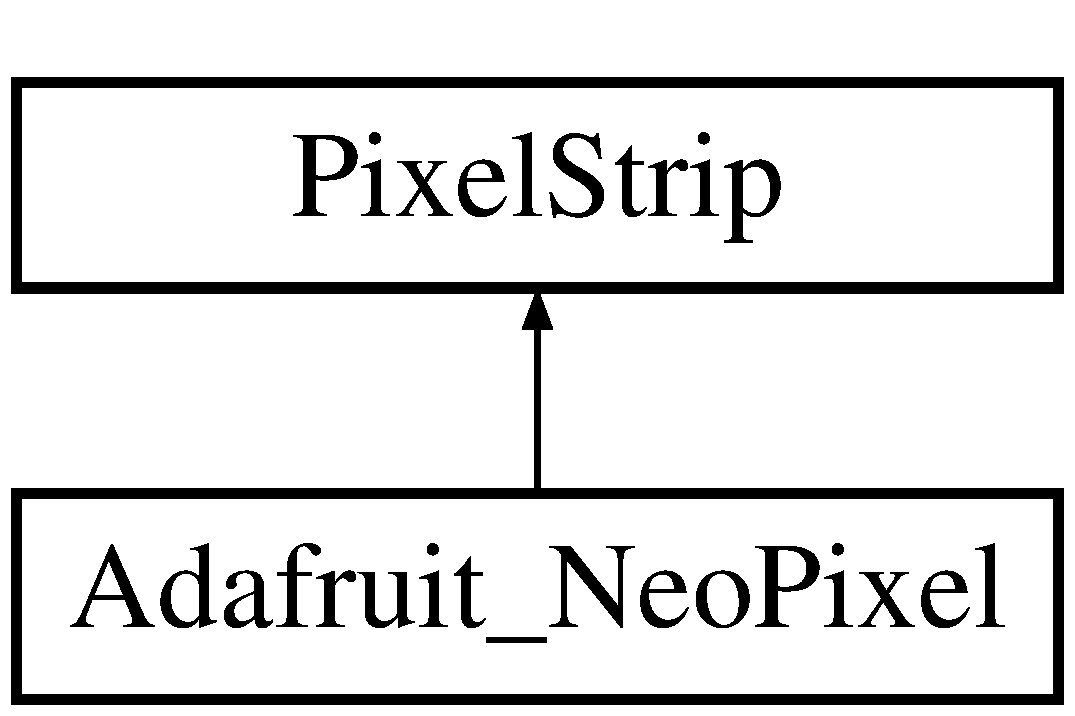
\includegraphics[height=2.000000cm]{class_adafruit___neo_pixel}
\end{center}
\end{figure}
\subsection*{Public Member Functions}
\begin{DoxyCompactItemize}
\item 
{\bf Adafruit\+\_\+\+Neo\+Pixel} (uint16\+\_\+t n, uint8\+\_\+t p=6, uint8\+\_\+t t=N\+E\+O\+\_\+\+G\+R\+B+N\+E\+O\+\_\+\+K\+H\+Z800)
\item 
void {\bf begin} (void)
\item 
void {\bf show} (void)
\item 
void {\bf set\+Pin} (uint8\+\_\+t p)
\item 
void {\bf set\+Pixel\+Color} (uint16\+\_\+t n, uint8\+\_\+t r, uint8\+\_\+t g, uint8\+\_\+t b)
\item 
void {\bf set\+Pixel\+Color} (uint16\+\_\+t n, uint32\+\_\+t c)
\item 
void {\bf set\+Brightness} (uint8\+\_\+t bright)
\item 
uint8\+\_\+t {\bf get\+Brightness} (void) const 
\item 
void {\bf clear} ()
\item 
uint8\+\_\+t $\ast$ {\bf get\+Pixels} (void) const 
\item 
uint16\+\_\+t {\bf num\+Pixels} (void) const 
\item 
uint32\+\_\+t {\bf get\+Pixel\+Color} (uint16\+\_\+t n) const 
\item 
bool {\bfseries can\+Show} (void)\label{class_adafruit___neo_pixel_a9e900a60b0ac2b43b99309bb118b929e}

\end{DoxyCompactItemize}
\subsection*{Static Public Member Functions}
\begin{DoxyCompactItemize}
\item 
static uint32\+\_\+t {\bf Color} (uint8\+\_\+t r, uint8\+\_\+t g, uint8\+\_\+t b)
\end{DoxyCompactItemize}


\subsection{Detailed Description}
Class for the physical Adafruit Neo\+Pixel panel products. 

\subsection{Constructor \& Destructor Documentation}
\index{Adafruit\+\_\+\+Neo\+Pixel@{Adafruit\+\_\+\+Neo\+Pixel}!Adafruit\+\_\+\+Neo\+Pixel@{Adafruit\+\_\+\+Neo\+Pixel}}
\index{Adafruit\+\_\+\+Neo\+Pixel@{Adafruit\+\_\+\+Neo\+Pixel}!Adafruit\+\_\+\+Neo\+Pixel@{Adafruit\+\_\+\+Neo\+Pixel}}
\subsubsection[{Adafruit\+\_\+\+Neo\+Pixel}]{\setlength{\rightskip}{0pt plus 5cm}Adafruit\+\_\+\+Neo\+Pixel\+::\+Adafruit\+\_\+\+Neo\+Pixel (
\begin{DoxyParamCaption}
\item[{uint16\+\_\+t}]{n, }
\item[{uint8\+\_\+t}]{p = {\ttfamily 6}, }
\item[{uint8\+\_\+t}]{t = {\ttfamily NEO\+\_\+GRB~+~NEO\+\_\+KHZ800}}
\end{DoxyParamCaption}
)}\label{class_adafruit___neo_pixel_ab8675c851ba6ee66407443faf36313f7}
Create a Neo\+Pixel Object 
\begin{DoxyParams}{Parameters}
{\em n} & Number of leds \\
\hline
{\em p} & Pin number \\
\hline
{\em t} & L\+E\+D type \\
\hline
\end{DoxyParams}


\subsection{Member Function Documentation}
\index{Adafruit\+\_\+\+Neo\+Pixel@{Adafruit\+\_\+\+Neo\+Pixel}!begin@{begin}}
\index{begin@{begin}!Adafruit\+\_\+\+Neo\+Pixel@{Adafruit\+\_\+\+Neo\+Pixel}}
\subsubsection[{begin}]{\setlength{\rightskip}{0pt plus 5cm}void Adafruit\+\_\+\+Neo\+Pixel\+::begin (
\begin{DoxyParamCaption}
\item[{void}]{}
\end{DoxyParamCaption}
)}\label{class_adafruit___neo_pixel_ac1cb16509be644232ce0e28d250083da}
Initialize the Neo\+Pixel \index{Adafruit\+\_\+\+Neo\+Pixel@{Adafruit\+\_\+\+Neo\+Pixel}!clear@{clear}}
\index{clear@{clear}!Adafruit\+\_\+\+Neo\+Pixel@{Adafruit\+\_\+\+Neo\+Pixel}}
\subsubsection[{clear}]{\setlength{\rightskip}{0pt plus 5cm}void Adafruit\+\_\+\+Neo\+Pixel\+::clear (
\begin{DoxyParamCaption}
{}
\end{DoxyParamCaption}
)\hspace{0.3cm}{\ttfamily [virtual]}}\label{class_adafruit___neo_pixel_ac06a711d7bf63bada61b52a1d528e4b4}
Sets all values to 0 (off) 

Implements {\bf Pixel\+Strip} \doxyref{}{p.}{class_pixel_strip_a9bc0c906bc3847c832e78af0c1afb6b8}.

\index{Adafruit\+\_\+\+Neo\+Pixel@{Adafruit\+\_\+\+Neo\+Pixel}!Color@{Color}}
\index{Color@{Color}!Adafruit\+\_\+\+Neo\+Pixel@{Adafruit\+\_\+\+Neo\+Pixel}}
\subsubsection[{Color}]{\setlength{\rightskip}{0pt plus 5cm}uint32\+\_\+t Adafruit\+\_\+\+Neo\+Pixel\+::\+Color (
\begin{DoxyParamCaption}
\item[{uint8\+\_\+t}]{r, }
\item[{uint8\+\_\+t}]{g, }
\item[{uint8\+\_\+t}]{b}
\end{DoxyParamCaption}
)\hspace{0.3cm}{\ttfamily [static]}}\label{class_adafruit___neo_pixel_ac49f3c50948815d45cecccbc66453386}
Convert separate R,G,B into packed 32-\/bit R\+G\+B color. Packed format is always R\+G\+B, regardless of L\+E\+D strand color order. \index{Adafruit\+\_\+\+Neo\+Pixel@{Adafruit\+\_\+\+Neo\+Pixel}!get\+Brightness@{get\+Brightness}}
\index{get\+Brightness@{get\+Brightness}!Adafruit\+\_\+\+Neo\+Pixel@{Adafruit\+\_\+\+Neo\+Pixel}}
\subsubsection[{get\+Brightness}]{\setlength{\rightskip}{0pt plus 5cm}uint8\+\_\+t Adafruit\+\_\+\+Neo\+Pixel\+::get\+Brightness (
\begin{DoxyParamCaption}
\item[{void}]{}
\end{DoxyParamCaption}
) const\hspace{0.3cm}{\ttfamily [virtual]}}\label{class_adafruit___neo_pixel_a3e3dc79b4fad55ea34799c6fa5f8cb82}
Return the brightness value 

Implements {\bf Pixel\+Strip} \doxyref{}{p.}{class_pixel_strip_aa79c0e3c07e10f0c5c6cd4fb9d1a60ab}.

\index{Adafruit\+\_\+\+Neo\+Pixel@{Adafruit\+\_\+\+Neo\+Pixel}!get\+Pixel\+Color@{get\+Pixel\+Color}}
\index{get\+Pixel\+Color@{get\+Pixel\+Color}!Adafruit\+\_\+\+Neo\+Pixel@{Adafruit\+\_\+\+Neo\+Pixel}}
\subsubsection[{get\+Pixel\+Color}]{\setlength{\rightskip}{0pt plus 5cm}uint32\+\_\+t Adafruit\+\_\+\+Neo\+Pixel\+::get\+Pixel\+Color (
\begin{DoxyParamCaption}
\item[{uint16\+\_\+t}]{n}
\end{DoxyParamCaption}
) const\hspace{0.3cm}{\ttfamily [virtual]}}\label{class_adafruit___neo_pixel_a309cd3fb7a3e2e87a26e7a2fcf6391f1}
Query color from previously-\/set pixel (returns packed 32-\/bit R\+G\+B value) 

Implements {\bf Pixel\+Strip} \doxyref{}{p.}{class_pixel_strip_a273498bf50216a646f24876da0e8d333}.

\index{Adafruit\+\_\+\+Neo\+Pixel@{Adafruit\+\_\+\+Neo\+Pixel}!get\+Pixels@{get\+Pixels}}
\index{get\+Pixels@{get\+Pixels}!Adafruit\+\_\+\+Neo\+Pixel@{Adafruit\+\_\+\+Neo\+Pixel}}
\subsubsection[{get\+Pixels}]{\setlength{\rightskip}{0pt plus 5cm}uint8\+\_\+t $\ast$ Adafruit\+\_\+\+Neo\+Pixel\+::get\+Pixels (
\begin{DoxyParamCaption}
\item[{void}]{}
\end{DoxyParamCaption}
) const}\label{class_adafruit___neo_pixel_a7ece3071ea718d37308f7a31fe82637c}
Returns pointer to pixels[] array. Pixel data is stored in device-\/ native format and is not translated here. Application will need to be aware whether pixels are R\+G\+B vs. G\+R\+B and handle colors appropriately. \index{Adafruit\+\_\+\+Neo\+Pixel@{Adafruit\+\_\+\+Neo\+Pixel}!num\+Pixels@{num\+Pixels}}
\index{num\+Pixels@{num\+Pixels}!Adafruit\+\_\+\+Neo\+Pixel@{Adafruit\+\_\+\+Neo\+Pixel}}
\subsubsection[{num\+Pixels}]{\setlength{\rightskip}{0pt plus 5cm}uint16\+\_\+t Adafruit\+\_\+\+Neo\+Pixel\+::num\+Pixels (
\begin{DoxyParamCaption}
\item[{void}]{}
\end{DoxyParamCaption}
) const\hspace{0.3cm}{\ttfamily [virtual]}}\label{class_adafruit___neo_pixel_a2b2ec05493af8de2a6afe63c1e8f9516}
Get the number of pixels this strip was initialized to. 

Implements {\bf Pixel\+Strip} \doxyref{}{p.}{class_pixel_strip_a095201c971095020d1adc10b094c896f}.

\index{Adafruit\+\_\+\+Neo\+Pixel@{Adafruit\+\_\+\+Neo\+Pixel}!set\+Brightness@{set\+Brightness}}
\index{set\+Brightness@{set\+Brightness}!Adafruit\+\_\+\+Neo\+Pixel@{Adafruit\+\_\+\+Neo\+Pixel}}
\subsubsection[{set\+Brightness}]{\setlength{\rightskip}{0pt plus 5cm}void Adafruit\+\_\+\+Neo\+Pixel\+::set\+Brightness (
\begin{DoxyParamCaption}
\item[{uint8\+\_\+t}]{bright}
\end{DoxyParamCaption}
)\hspace{0.3cm}{\ttfamily [virtual]}}\label{class_adafruit___neo_pixel_a06915c54a2cc307763b3c44a601229ba}
Adjust output brightness; This does N\+O\+T immediately affect what\textquotesingle{}s currently displayed on the L\+E\+Ds. The next call to \doxyref{show()}{p.}{class_adafruit___neo_pixel_a4bcda7a15591065570d3598cbf970be7} will refresh the L\+E\+Ds at this level. However, this process is potentially \char`\"{}lossy,\char`\"{} especially when increasing brightness. The tight timing in the W\+S2811/\+W\+S2812 code means there aren\textquotesingle{}t enough free cycles to perform this scaling on the fly as data is issued. So we make a pass through the existing color data in R\+A\+M and scale it (subsequent graphics commands also work at this brightness level). If there\textquotesingle{}s a significant step up in brightness, the limited number of steps (quantization) in the old data will be quite visible in the re-\/scaled version. For a non-\/destructive change, you\textquotesingle{}ll need to re-\/render the full strip data. C\textquotesingle{}est la vie. 
\begin{DoxyParams}{Parameters}
{\em bright} & 0=darkest (off), 255=brightest. \\
\hline
\end{DoxyParams}


Implements {\bf Pixel\+Strip} \doxyref{}{p.}{class_pixel_strip_a3154e9d623c7ffc39dd70f6cfd39bd68}.

\index{Adafruit\+\_\+\+Neo\+Pixel@{Adafruit\+\_\+\+Neo\+Pixel}!set\+Pin@{set\+Pin}}
\index{set\+Pin@{set\+Pin}!Adafruit\+\_\+\+Neo\+Pixel@{Adafruit\+\_\+\+Neo\+Pixel}}
\subsubsection[{set\+Pin}]{\setlength{\rightskip}{0pt plus 5cm}void Adafruit\+\_\+\+Neo\+Pixel\+::set\+Pin (
\begin{DoxyParamCaption}
\item[{uint8\+\_\+t}]{p}
\end{DoxyParamCaption}
)}\label{class_adafruit___neo_pixel_a64a6704fdac239046791e7a9f7a76ab6}
Set the output pin number \index{Adafruit\+\_\+\+Neo\+Pixel@{Adafruit\+\_\+\+Neo\+Pixel}!set\+Pixel\+Color@{set\+Pixel\+Color}}
\index{set\+Pixel\+Color@{set\+Pixel\+Color}!Adafruit\+\_\+\+Neo\+Pixel@{Adafruit\+\_\+\+Neo\+Pixel}}
\subsubsection[{set\+Pixel\+Color}]{\setlength{\rightskip}{0pt plus 5cm}void Adafruit\+\_\+\+Neo\+Pixel\+::set\+Pixel\+Color (
\begin{DoxyParamCaption}
\item[{uint16\+\_\+t}]{n, }
\item[{uint8\+\_\+t}]{r, }
\item[{uint8\+\_\+t}]{g, }
\item[{uint8\+\_\+t}]{b}
\end{DoxyParamCaption}
)\hspace{0.3cm}{\ttfamily [virtual]}}\label{class_adafruit___neo_pixel_ab8763ccc6f9a090df1f753905fd5561e}
Set pixel color from separate R,G,B components\+: 
\begin{DoxyParams}{Parameters}
{\em n} & Pixel number \\
\hline
{\em r} & Red component (0-\/255 \\
\hline
{\em g} & Green component \\
\hline
{\em b} & Blue component \\
\hline
\end{DoxyParams}


Implements {\bf Pixel\+Strip} \doxyref{}{p.}{class_pixel_strip_a391a297d5f9faf1be384bada7199acce}.

\index{Adafruit\+\_\+\+Neo\+Pixel@{Adafruit\+\_\+\+Neo\+Pixel}!set\+Pixel\+Color@{set\+Pixel\+Color}}
\index{set\+Pixel\+Color@{set\+Pixel\+Color}!Adafruit\+\_\+\+Neo\+Pixel@{Adafruit\+\_\+\+Neo\+Pixel}}
\subsubsection[{set\+Pixel\+Color}]{\setlength{\rightskip}{0pt plus 5cm}void Adafruit\+\_\+\+Neo\+Pixel\+::set\+Pixel\+Color (
\begin{DoxyParamCaption}
\item[{uint16\+\_\+t}]{n, }
\item[{uint32\+\_\+t}]{c}
\end{DoxyParamCaption}
)\hspace{0.3cm}{\ttfamily [virtual]}}\label{class_adafruit___neo_pixel_a19fc274330c0e65907929ee03b93b1c3}
Set pixel color from \textquotesingle{}packed\textquotesingle{} 32-\/bit R\+G\+B color\+: 

Implements {\bf Pixel\+Strip} \doxyref{}{p.}{class_pixel_strip_a8fac5124e323b48aaa854143d0d91922}.

\index{Adafruit\+\_\+\+Neo\+Pixel@{Adafruit\+\_\+\+Neo\+Pixel}!show@{show}}
\index{show@{show}!Adafruit\+\_\+\+Neo\+Pixel@{Adafruit\+\_\+\+Neo\+Pixel}}
\subsubsection[{show}]{\setlength{\rightskip}{0pt plus 5cm}void Adafruit\+\_\+\+Neo\+Pixel\+::show (
\begin{DoxyParamCaption}
\item[{void}]{}
\end{DoxyParamCaption}
)}\label{class_adafruit___neo_pixel_a4bcda7a15591065570d3598cbf970be7}
Refresh the data into the Neo\+Pixel. This needs to be called to display the current data. 

The documentation for this class was generated from the following files\+:\begin{DoxyCompactItemize}
\item 
C\+:/\+Users/\+Russell/\+Documents/\+Arduino/libraries/\+Opcom\+\_\+\+Neo\+Pixel/Adafruit\+\_\+\+Neo\+Pixel.\+h\item 
C\+:/\+Users/\+Russell/\+Documents/\+Arduino/libraries/\+Opcom\+\_\+\+Neo\+Pixel/Adafruit\+\_\+\+Neo\+Pixel.\+cpp\end{DoxyCompactItemize}

\section{P\+E\+Node Struct Reference}
\label{struct_p_e_node}\index{P\+E\+Node@{P\+E\+Node}}


{\ttfamily \#include $<$Pixel\+Effect\+Stack.\+h$>$}

\subsection*{Public Attributes}
\begin{DoxyCompactItemize}
\item 
{\bf Pixel\+Effect} $\ast$ {\bf effect}
\item 
{\bf P\+E\+Node} $\ast$ {\bf next}
\end{DoxyCompactItemize}


\subsection{Detailed Description}
Linked list of effects 

\subsection{Member Data Documentation}
\index{P\+E\+Node@{P\+E\+Node}!effect@{effect}}
\index{effect@{effect}!P\+E\+Node@{P\+E\+Node}}
\subsubsection[{effect}]{\setlength{\rightskip}{0pt plus 5cm}{\bf Pixel\+Effect}$\ast$ P\+E\+Node\+::effect}\label{struct_p_e_node_a591d88d783fdb83bfb32b1590a1d1152}
effect pointer \index{P\+E\+Node@{P\+E\+Node}!next@{next}}
\index{next@{next}!P\+E\+Node@{P\+E\+Node}}
\subsubsection[{next}]{\setlength{\rightskip}{0pt plus 5cm}{\bf P\+E\+Node}$\ast$ P\+E\+Node\+::next}\label{struct_p_e_node_af10ed8847b32092d7b81103edd83b270}
pointer to next item in list 

The documentation for this struct was generated from the following file\+:\begin{DoxyCompactItemize}
\item 
C\+:/\+Users/\+Russell/\+Documents/\+Arduino/libraries/\+Opcom\+\_\+\+Neo\+Pixel/Pixel\+Effect\+Stack.\+h\end{DoxyCompactItemize}

\section{Pixel\+Effect Class Reference}
\label{class_pixel_effect}\index{Pixel\+Effect@{Pixel\+Effect}}


{\ttfamily \#include $<$Pixel\+Effect.\+h$>$}

Inheritance diagram for Pixel\+Effect\+:\begin{figure}[H]
\begin{center}
\leavevmode
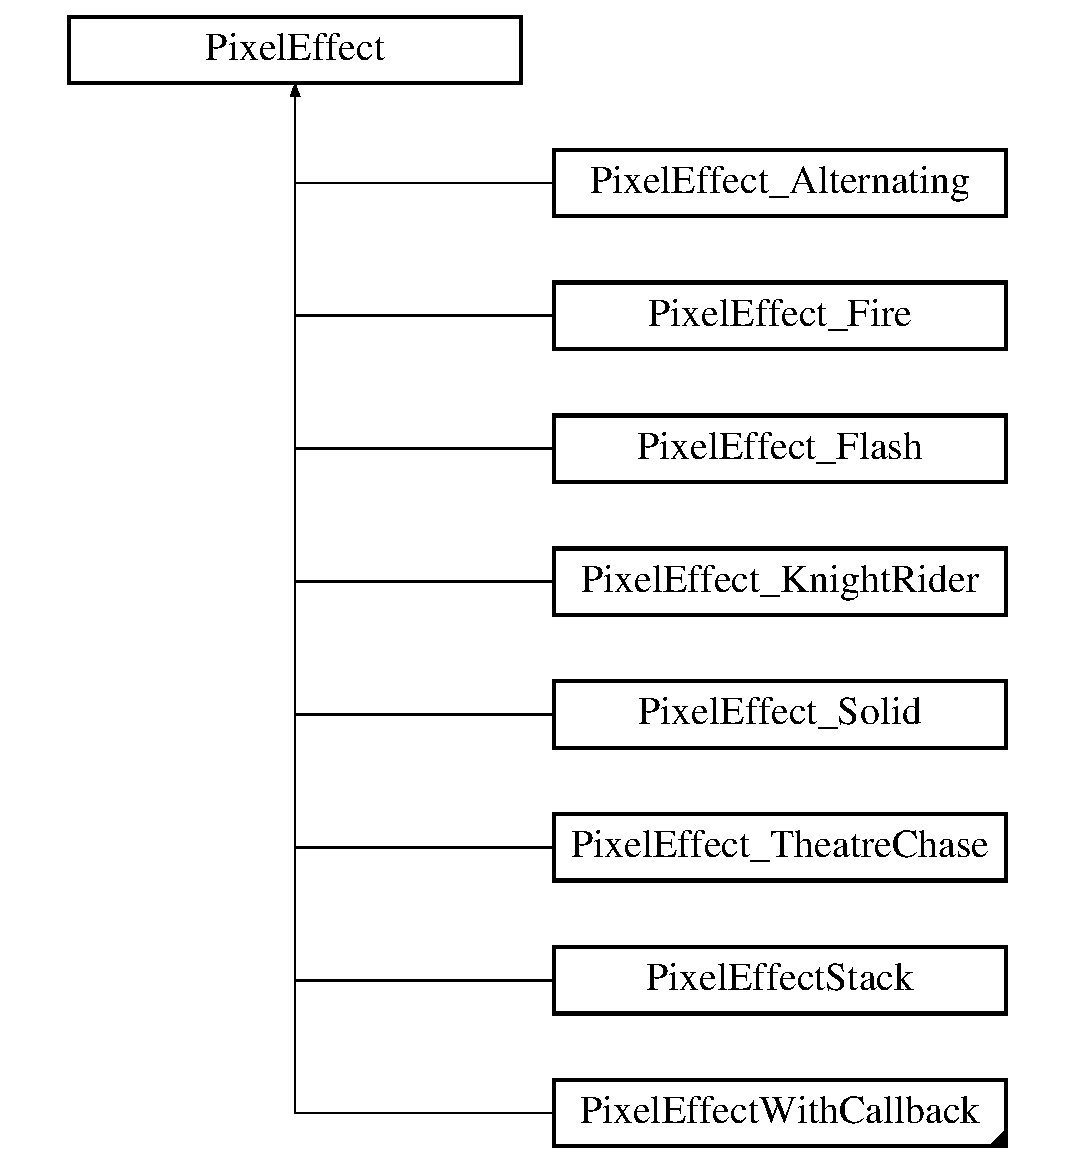
\includegraphics[height=9.000000cm]{class_pixel_effect}
\end{center}
\end{figure}
\subsection*{Public Member Functions}
\begin{DoxyCompactItemize}
\item 
void {\bf disable} ()
\item 
void {\bf enable} ()
\item 
bool {\bf is\+Enabled} ()
\item 
virtual void {\bf init} ()=0
\item 
virtual void {\bf run} ()=0
\end{DoxyCompactItemize}
\subsection*{Protected Member Functions}
\begin{DoxyCompactItemize}
\item 
{\bf Pixel\+Effect} ({\bf Pixel\+Strip} $\ast$strip)
\end{DoxyCompactItemize}
\subsection*{Protected Attributes}
\begin{DoxyCompactItemize}
\item 
{\bf Pixel\+Strip} $\ast$ {\bf m\+\_\+strip}
\item 
bool {\bf m\+\_\+enabled}
\end{DoxyCompactItemize}


\subsection{Detailed Description}
The base class for any light effect. Light effects can be added to either a physical \doxyref{Pixel\+Strip}{p.}{class_pixel_strip} or a \doxyref{Pixel\+Panel}{p.}{class_pixel_panel} 

\subsection{Constructor \& Destructor Documentation}
\index{Pixel\+Effect@{Pixel\+Effect}!Pixel\+Effect@{Pixel\+Effect}}
\index{Pixel\+Effect@{Pixel\+Effect}!Pixel\+Effect@{Pixel\+Effect}}
\subsubsection[{Pixel\+Effect}]{\setlength{\rightskip}{0pt plus 5cm}Pixel\+Effect\+::\+Pixel\+Effect (
\begin{DoxyParamCaption}
\item[{{\bf Pixel\+Strip} $\ast$}]{strip}
\end{DoxyParamCaption}
)\hspace{0.3cm}{\ttfamily [inline]}, {\ttfamily [protected]}}\label{class_pixel_effect_a1d090e3203685f2eb92d37404fc823e5}
Should be called by sub classes. Sets up the strip and enables the effect by default. 
\begin{DoxyParams}{Parameters}
{\em strip} & Physical strip or logical Panel pointer \\
\hline
\end{DoxyParams}


\subsection{Member Function Documentation}
\index{Pixel\+Effect@{Pixel\+Effect}!disable@{disable}}
\index{disable@{disable}!Pixel\+Effect@{Pixel\+Effect}}
\subsubsection[{disable}]{\setlength{\rightskip}{0pt plus 5cm}void Pixel\+Effect\+::disable (
\begin{DoxyParamCaption}
{}
\end{DoxyParamCaption}
)\hspace{0.3cm}{\ttfamily [inline]}}\label{class_pixel_effect_ac5f4105763604a3b44c28d7eec34885e}
Disable running. This will prevent the light effect from updating during the call to \doxyref{run()}{p.}{class_pixel_effect_adfff257c93348ebca93bcc7f38eee20d} \index{Pixel\+Effect@{Pixel\+Effect}!enable@{enable}}
\index{enable@{enable}!Pixel\+Effect@{Pixel\+Effect}}
\subsubsection[{enable}]{\setlength{\rightskip}{0pt plus 5cm}void Pixel\+Effect\+::enable (
\begin{DoxyParamCaption}
{}
\end{DoxyParamCaption}
)\hspace{0.3cm}{\ttfamily [inline]}}\label{class_pixel_effect_a97987697b6f5cce2a522d7936441e2aa}
Enable running. This will cause the light effect to be updated during the call to \doxyref{run()}{p.}{class_pixel_effect_adfff257c93348ebca93bcc7f38eee20d} \index{Pixel\+Effect@{Pixel\+Effect}!init@{init}}
\index{init@{init}!Pixel\+Effect@{Pixel\+Effect}}
\subsubsection[{init}]{\setlength{\rightskip}{0pt plus 5cm}virtual void Pixel\+Effect\+::init (
\begin{DoxyParamCaption}
{}
\end{DoxyParamCaption}
)\hspace{0.3cm}{\ttfamily [pure virtual]}}\label{class_pixel_effect_ab3c11ba2c2f1cd26e62a0a8f16c6c02b}
The init function, which must be called before the effect is \doxyref{run()}{p.}{class_pixel_effect_adfff257c93348ebca93bcc7f38eee20d} 

Implemented in {\bf Pixel\+Effect\+Stack} \doxyref{}{p.}{class_pixel_effect_stack_a726083b8f63898358945226fa175757b}, {\bf Pixel\+Effect\+\_\+\+Knight\+Rider} \doxyref{}{p.}{class_pixel_effect___knight_rider_a16b3569280331671f795e367b4f4dd54}, {\bf Pixel\+Effect\+\_\+\+Color\+Wipe} \doxyref{}{p.}{class_pixel_effect___color_wipe_a29c4790d9b4ae6387d39f61963e57c5c}, {\bf Pixel\+Effect\+\_\+\+Fire} \doxyref{}{p.}{class_pixel_effect___fire_a210a5c79036f523f1a98fbf97a975d16}, {\bf Pixel\+Effect\+\_\+\+Flash} \doxyref{}{p.}{class_pixel_effect___flash_a4563d09b05c4af920675f7246d136c27}, {\bf Pixel\+Effect\+\_\+\+Theatre\+Chase} \doxyref{}{p.}{class_pixel_effect___theatre_chase_a6576f90406a69407d9b6633b30e1075e}, {\bf Pixel\+Effect\+\_\+\+Alternating} \doxyref{}{p.}{class_pixel_effect___alternating_a858035d6d8874e619289aae06078b4c0}, {\bf Pixel\+Effect\+\_\+\+Fade} \doxyref{}{p.}{class_pixel_effect___fade_a4a9ec0355f7afec0967d446a0b70a4d5}, and {\bf Pixel\+Effect\+\_\+\+Solid} \doxyref{}{p.}{class_pixel_effect___solid_a74c03fc565fde97566240ea176b7b5ce}.

\index{Pixel\+Effect@{Pixel\+Effect}!is\+Enabled@{is\+Enabled}}
\index{is\+Enabled@{is\+Enabled}!Pixel\+Effect@{Pixel\+Effect}}
\subsubsection[{is\+Enabled}]{\setlength{\rightskip}{0pt plus 5cm}bool Pixel\+Effect\+::is\+Enabled (
\begin{DoxyParamCaption}
{}
\end{DoxyParamCaption}
)\hspace{0.3cm}{\ttfamily [inline]}}\label{class_pixel_effect_a5e5f1c4df8f226b20a1efb859e0037c8}
Check if this light effect is enabled or not. \begin{DoxyReturn}{Returns}
True if enabled 
\end{DoxyReturn}
\index{Pixel\+Effect@{Pixel\+Effect}!run@{run}}
\index{run@{run}!Pixel\+Effect@{Pixel\+Effect}}
\subsubsection[{run}]{\setlength{\rightskip}{0pt plus 5cm}virtual void Pixel\+Effect\+::run (
\begin{DoxyParamCaption}
{}
\end{DoxyParamCaption}
)\hspace{0.3cm}{\ttfamily [pure virtual]}}\label{class_pixel_effect_adfff257c93348ebca93bcc7f38eee20d}
The \doxyref{run()}{p.}{class_pixel_effect_adfff257c93348ebca93bcc7f38eee20d} function, which is called to update the state of the light effect 

Implemented in {\bf Pixel\+Effect\+Stack} \doxyref{}{p.}{class_pixel_effect_stack_a6fbd31bab015a7d3526915a60392cbd1}, {\bf Pixel\+Effect\+\_\+\+Knight\+Rider} \doxyref{}{p.}{class_pixel_effect___knight_rider_a35c58ed5e875365942e4666d43eafe39}, {\bf Pixel\+Effect\+\_\+\+Color\+Wipe} \doxyref{}{p.}{class_pixel_effect___color_wipe_a86123dfb5f720e46f668e60a19f8808a}, {\bf Pixel\+Effect\+\_\+\+Fire} \doxyref{}{p.}{class_pixel_effect___fire_ac3d39af015e7005f8e345cc4d83d81f0}, {\bf Pixel\+Effect\+\_\+\+Flash} \doxyref{}{p.}{class_pixel_effect___flash_a96a43629b9422fc10420ab48604e08e2}, {\bf Pixel\+Effect\+\_\+\+Theatre\+Chase} \doxyref{}{p.}{class_pixel_effect___theatre_chase_a18283d29998b59918d604893cd3e9527}, {\bf Pixel\+Effect\+\_\+\+Alternating} \doxyref{}{p.}{class_pixel_effect___alternating_a14628ae24a18b1b9523dfb7e958a0712}, {\bf Pixel\+Effect\+\_\+\+Fade} \doxyref{}{p.}{class_pixel_effect___fade_ad538d7242223524b00c39104e2bc5001}, and {\bf Pixel\+Effect\+\_\+\+Solid} \doxyref{}{p.}{class_pixel_effect___solid_a2a5887f47c4f56d23707387be85d5b6b}.



\subsection{Member Data Documentation}
\index{Pixel\+Effect@{Pixel\+Effect}!m\+\_\+enabled@{m\+\_\+enabled}}
\index{m\+\_\+enabled@{m\+\_\+enabled}!Pixel\+Effect@{Pixel\+Effect}}
\subsubsection[{m\+\_\+enabled}]{\setlength{\rightskip}{0pt plus 5cm}bool Pixel\+Effect\+::m\+\_\+enabled\hspace{0.3cm}{\ttfamily [protected]}}\label{class_pixel_effect_a554bf74c717d48563aed3871c9e2bdc1}
true if effect is enabled and should be updated during run \index{Pixel\+Effect@{Pixel\+Effect}!m\+\_\+strip@{m\+\_\+strip}}
\index{m\+\_\+strip@{m\+\_\+strip}!Pixel\+Effect@{Pixel\+Effect}}
\subsubsection[{m\+\_\+strip}]{\setlength{\rightskip}{0pt plus 5cm}{\bf Pixel\+Strip}$\ast$ Pixel\+Effect\+::m\+\_\+strip\hspace{0.3cm}{\ttfamily [protected]}}\label{class_pixel_effect_af2e843ef8269aba69904f223773972ca}
The panel or strip this effect is running on 

The documentation for this class was generated from the following file\+:\begin{DoxyCompactItemize}
\item 
C\+:/\+Users/\+Russell/\+Documents/\+Arduino/libraries/\+Opcom\+\_\+\+Neo\+Pixel/Pixel\+Effect.\+h\end{DoxyCompactItemize}

\section{Pixel\+Effect\+\_\+\+Alternating Class Reference}
\label{class_pixel_effect___alternating}\index{Pixel\+Effect\+\_\+\+Alternating@{Pixel\+Effect\+\_\+\+Alternating}}


{\ttfamily \#include $<$Pixel\+Effect\+\_\+\+Alternating.\+h$>$}

Inheritance diagram for Pixel\+Effect\+\_\+\+Alternating\+:\begin{figure}[H]
\begin{center}
\leavevmode
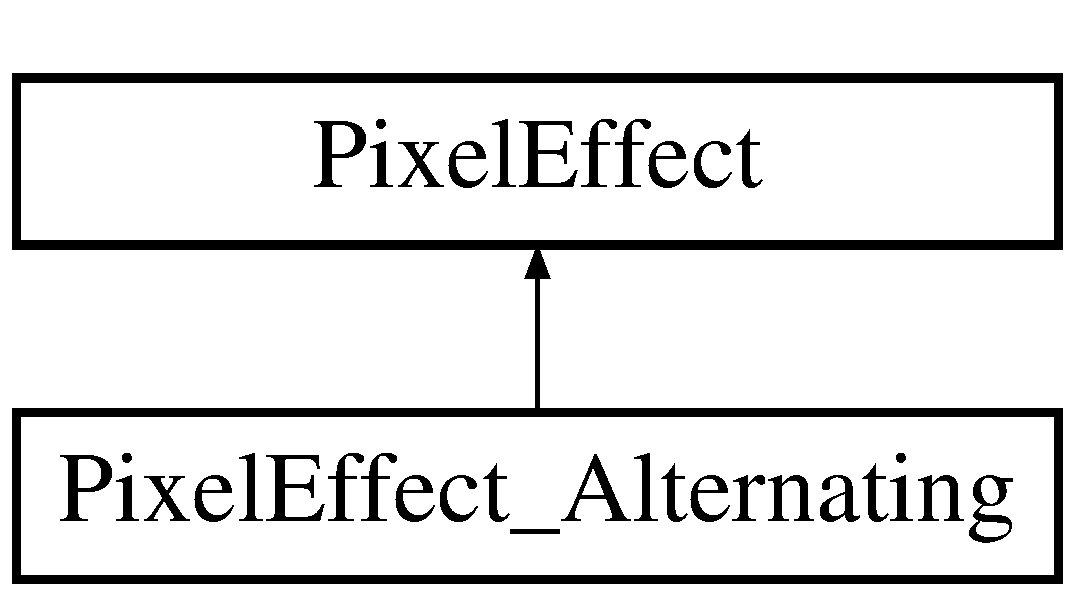
\includegraphics[height=2.000000cm]{class_pixel_effect___alternating}
\end{center}
\end{figure}
\subsection*{Public Member Functions}
\begin{DoxyCompactItemize}
\item 
{\bf Pixel\+Effect\+\_\+\+Alternating} ({\bf Pixel\+Strip} $\ast$strip, uint32\+\_\+t color, uint16\+\_\+t wait, uint32\+\_\+t color2=0)
\item 
void {\bf init} ()
\item 
void {\bf run} ()
\end{DoxyCompactItemize}
\subsection*{Additional Inherited Members}


\subsection{Detailed Description}
Alternating colors 

\subsection{Constructor \& Destructor Documentation}
\index{Pixel\+Effect\+\_\+\+Alternating@{Pixel\+Effect\+\_\+\+Alternating}!Pixel\+Effect\+\_\+\+Alternating@{Pixel\+Effect\+\_\+\+Alternating}}
\index{Pixel\+Effect\+\_\+\+Alternating@{Pixel\+Effect\+\_\+\+Alternating}!Pixel\+Effect\+\_\+\+Alternating@{Pixel\+Effect\+\_\+\+Alternating}}
\subsubsection[{Pixel\+Effect\+\_\+\+Alternating}]{\setlength{\rightskip}{0pt plus 5cm}Pixel\+Effect\+\_\+\+Alternating\+::\+Pixel\+Effect\+\_\+\+Alternating (
\begin{DoxyParamCaption}
\item[{{\bf Pixel\+Strip} $\ast$}]{strip, }
\item[{uint32\+\_\+t}]{color, }
\item[{uint16\+\_\+t}]{wait, }
\item[{uint32\+\_\+t}]{color2 = {\ttfamily 0}}
\end{DoxyParamCaption}
)\hspace{0.3cm}{\ttfamily [inline]}}\label{class_pixel_effect___alternating_af7247d2f1e8e7e01f8a7b5215a9ba7a5}
Alternate between two colors. 
\begin{DoxyParams}{Parameters}
{\em strip} & Physical strip or logical Panel pointer \\
\hline
{\em color} & Foreground (on) R\+G\+B color to display \\
\hline
{\em wait} & Milliseconds to pause between changing \\
\hline
{\em color2} & Background (off) color to display. Defaults to black (off) \\
\hline
\end{DoxyParams}


\subsection{Member Function Documentation}
\index{Pixel\+Effect\+\_\+\+Alternating@{Pixel\+Effect\+\_\+\+Alternating}!init@{init}}
\index{init@{init}!Pixel\+Effect\+\_\+\+Alternating@{Pixel\+Effect\+\_\+\+Alternating}}
\subsubsection[{init}]{\setlength{\rightskip}{0pt plus 5cm}void Pixel\+Effect\+\_\+\+Alternating\+::init (
\begin{DoxyParamCaption}
{}
\end{DoxyParamCaption}
)\hspace{0.3cm}{\ttfamily [inline]}, {\ttfamily [virtual]}}\label{class_pixel_effect___alternating_a858035d6d8874e619289aae06078b4c0}
The init function, which must be called before the effect is \doxyref{run()}{p.}{class_pixel_effect___alternating_a14628ae24a18b1b9523dfb7e958a0712} 

Implements {\bf Pixel\+Effect} \doxyref{}{p.}{class_pixel_effect_ab3c11ba2c2f1cd26e62a0a8f16c6c02b}.

\index{Pixel\+Effect\+\_\+\+Alternating@{Pixel\+Effect\+\_\+\+Alternating}!run@{run}}
\index{run@{run}!Pixel\+Effect\+\_\+\+Alternating@{Pixel\+Effect\+\_\+\+Alternating}}
\subsubsection[{run}]{\setlength{\rightskip}{0pt plus 5cm}void Pixel\+Effect\+\_\+\+Alternating\+::run (
\begin{DoxyParamCaption}
{}
\end{DoxyParamCaption}
)\hspace{0.3cm}{\ttfamily [inline]}, {\ttfamily [virtual]}}\label{class_pixel_effect___alternating_a14628ae24a18b1b9523dfb7e958a0712}
The \doxyref{run()}{p.}{class_pixel_effect___alternating_a14628ae24a18b1b9523dfb7e958a0712} function, which is called to update the state of the light effect 

Implements {\bf Pixel\+Effect} \doxyref{}{p.}{class_pixel_effect_adfff257c93348ebca93bcc7f38eee20d}.



The documentation for this class was generated from the following file\+:\begin{DoxyCompactItemize}
\item 
C\+:/\+Users/\+Russell/\+Documents/\+Arduino/libraries/\+Opcom\+\_\+\+Neo\+Pixel/Pixel\+Effect\+\_\+\+Alternating.\+h\end{DoxyCompactItemize}

\section{Pixel\+Effect\+\_\+\+Color\+Wipe Class Reference}
\label{class_pixel_effect___color_wipe}\index{Pixel\+Effect\+\_\+\+Color\+Wipe@{Pixel\+Effect\+\_\+\+Color\+Wipe}}


{\ttfamily \#include $<$Pixel\+Effect\+\_\+\+Color\+Wipe.\+h$>$}

Inheritance diagram for Pixel\+Effect\+\_\+\+Color\+Wipe\+:\begin{figure}[H]
\begin{center}
\leavevmode
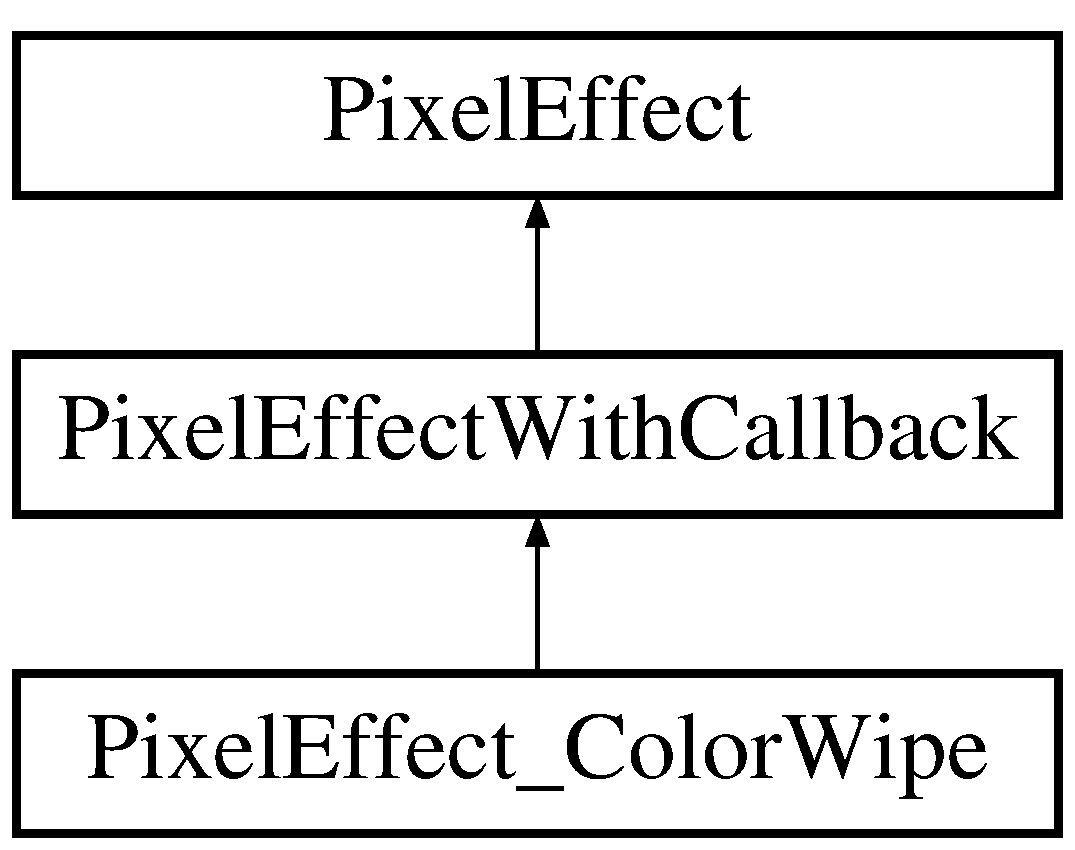
\includegraphics[height=3.000000cm]{class_pixel_effect___color_wipe}
\end{center}
\end{figure}
\subsection*{Public Member Functions}
\begin{DoxyCompactItemize}
\item 
{\bf Pixel\+Effect\+\_\+\+Color\+Wipe} ({\bf Pixel\+Strip} $\ast$strip, uint32\+\_\+t color, uint32\+\_\+t delay)
\item 
void {\bf set\+Clear\+Background} (bool v)
\item 
void {\bf set\+Filled\+Delay} (uint32\+\_\+t delay)
\item 
void {\bf init} ()
\item 
void {\bf run} ()
\end{DoxyCompactItemize}
\subsection*{Additional Inherited Members}


\subsection{Detailed Description}
A color wipe that fills strip pixel by pixel. Defaults to immediately clearing and starting a new wipe.

The cb\+Init function is called each time the effect starts over, before clearing the panel. cb\+Finished is called once the panel is full, after the pixels have displayed for the on time. Return false from cb\+Finished to stop the display from being cleared. 

\subsection{Constructor \& Destructor Documentation}
\index{Pixel\+Effect\+\_\+\+Color\+Wipe@{Pixel\+Effect\+\_\+\+Color\+Wipe}!Pixel\+Effect\+\_\+\+Color\+Wipe@{Pixel\+Effect\+\_\+\+Color\+Wipe}}
\index{Pixel\+Effect\+\_\+\+Color\+Wipe@{Pixel\+Effect\+\_\+\+Color\+Wipe}!Pixel\+Effect\+\_\+\+Color\+Wipe@{Pixel\+Effect\+\_\+\+Color\+Wipe}}
\subsubsection[{Pixel\+Effect\+\_\+\+Color\+Wipe}]{\setlength{\rightskip}{0pt plus 5cm}Pixel\+Effect\+\_\+\+Color\+Wipe\+::\+Pixel\+Effect\+\_\+\+Color\+Wipe (
\begin{DoxyParamCaption}
\item[{{\bf Pixel\+Strip} $\ast$}]{strip, }
\item[{uint32\+\_\+t}]{color, }
\item[{uint32\+\_\+t}]{delay}
\end{DoxyParamCaption}
)\hspace{0.3cm}{\ttfamily [inline]}}\label{class_pixel_effect___color_wipe_a4a32c7e85ebd5c0ee452ff44bc8b73e5}
Wipe a color in to fill a strip 
\begin{DoxyParams}{Parameters}
{\em strip} & Pixel panel \\
\hline
{\em color} & Foreground color for fill \\
\hline
{\em delay} & milliseconds between pixels \\
\hline
\end{DoxyParams}


\subsection{Member Function Documentation}
\index{Pixel\+Effect\+\_\+\+Color\+Wipe@{Pixel\+Effect\+\_\+\+Color\+Wipe}!init@{init}}
\index{init@{init}!Pixel\+Effect\+\_\+\+Color\+Wipe@{Pixel\+Effect\+\_\+\+Color\+Wipe}}
\subsubsection[{init}]{\setlength{\rightskip}{0pt plus 5cm}void Pixel\+Effect\+\_\+\+Color\+Wipe\+::init (
\begin{DoxyParamCaption}
{}
\end{DoxyParamCaption}
)\hspace{0.3cm}{\ttfamily [inline]}, {\ttfamily [virtual]}}\label{class_pixel_effect___color_wipe_a29c4790d9b4ae6387d39f61963e57c5c}
The init function, which must be called before the effect is \doxyref{run()}{p.}{class_pixel_effect___color_wipe_a86123dfb5f720e46f668e60a19f8808a} 

Implements {\bf Pixel\+Effect} \doxyref{}{p.}{class_pixel_effect_ab3c11ba2c2f1cd26e62a0a8f16c6c02b}.

\index{Pixel\+Effect\+\_\+\+Color\+Wipe@{Pixel\+Effect\+\_\+\+Color\+Wipe}!run@{run}}
\index{run@{run}!Pixel\+Effect\+\_\+\+Color\+Wipe@{Pixel\+Effect\+\_\+\+Color\+Wipe}}
\subsubsection[{run}]{\setlength{\rightskip}{0pt plus 5cm}void Pixel\+Effect\+\_\+\+Color\+Wipe\+::run (
\begin{DoxyParamCaption}
{}
\end{DoxyParamCaption}
)\hspace{0.3cm}{\ttfamily [inline]}, {\ttfamily [virtual]}}\label{class_pixel_effect___color_wipe_a86123dfb5f720e46f668e60a19f8808a}
The \doxyref{run()}{p.}{class_pixel_effect___color_wipe_a86123dfb5f720e46f668e60a19f8808a} function, which is called to update the state of the light effect 

Implements {\bf Pixel\+Effect} \doxyref{}{p.}{class_pixel_effect_adfff257c93348ebca93bcc7f38eee20d}.

\index{Pixel\+Effect\+\_\+\+Color\+Wipe@{Pixel\+Effect\+\_\+\+Color\+Wipe}!set\+Clear\+Background@{set\+Clear\+Background}}
\index{set\+Clear\+Background@{set\+Clear\+Background}!Pixel\+Effect\+\_\+\+Color\+Wipe@{Pixel\+Effect\+\_\+\+Color\+Wipe}}
\subsubsection[{set\+Clear\+Background}]{\setlength{\rightskip}{0pt plus 5cm}void Pixel\+Effect\+\_\+\+Color\+Wipe\+::set\+Clear\+Background (
\begin{DoxyParamCaption}
\item[{bool}]{v}
\end{DoxyParamCaption}
)\hspace{0.3cm}{\ttfamily [inline]}}\label{class_pixel_effect___color_wipe_a155c115000794ec444163e31f1125a55}
Set to false if you do not wish the existing pixels cleared on first run. The strip will be cleared on each subsequent run regardless. 
\begin{DoxyParams}{Parameters}
{\em v} & True to clear background before first run \\
\hline
\end{DoxyParams}
\index{Pixel\+Effect\+\_\+\+Color\+Wipe@{Pixel\+Effect\+\_\+\+Color\+Wipe}!set\+Filled\+Delay@{set\+Filled\+Delay}}
\index{set\+Filled\+Delay@{set\+Filled\+Delay}!Pixel\+Effect\+\_\+\+Color\+Wipe@{Pixel\+Effect\+\_\+\+Color\+Wipe}}
\subsubsection[{set\+Filled\+Delay}]{\setlength{\rightskip}{0pt plus 5cm}void Pixel\+Effect\+\_\+\+Color\+Wipe\+::set\+Filled\+Delay (
\begin{DoxyParamCaption}
\item[{uint32\+\_\+t}]{delay}
\end{DoxyParamCaption}
)\hspace{0.3cm}{\ttfamily [inline]}}\label{class_pixel_effect___color_wipe_a5e45401882581dd4f4b2e93088f3ed98}
Set the delay at the end of the cycle when all the pixels have filled. By default this value is the same as the delay between pixels. 
\begin{DoxyParams}{Parameters}
{\em delay} & Delay time in ms \\
\hline
\end{DoxyParams}


The documentation for this class was generated from the following file\+:\begin{DoxyCompactItemize}
\item 
C\+:/\+Users/\+Russell/\+Documents/\+Arduino/libraries/\+Opcom\+\_\+\+Neo\+Pixel/Pixel\+Effect\+\_\+\+Color\+Wipe.\+h\end{DoxyCompactItemize}

\section{Pixel\+Effect\+\_\+\+Fade Class Reference}
\label{class_pixel_effect___fade}\index{Pixel\+Effect\+\_\+\+Fade@{Pixel\+Effect\+\_\+\+Fade}}


{\ttfamily \#include $<$Pixel\+Effect\+\_\+\+Fade.\+h$>$}

Inheritance diagram for Pixel\+Effect\+\_\+\+Fade\+:\begin{figure}[H]
\begin{center}
\leavevmode
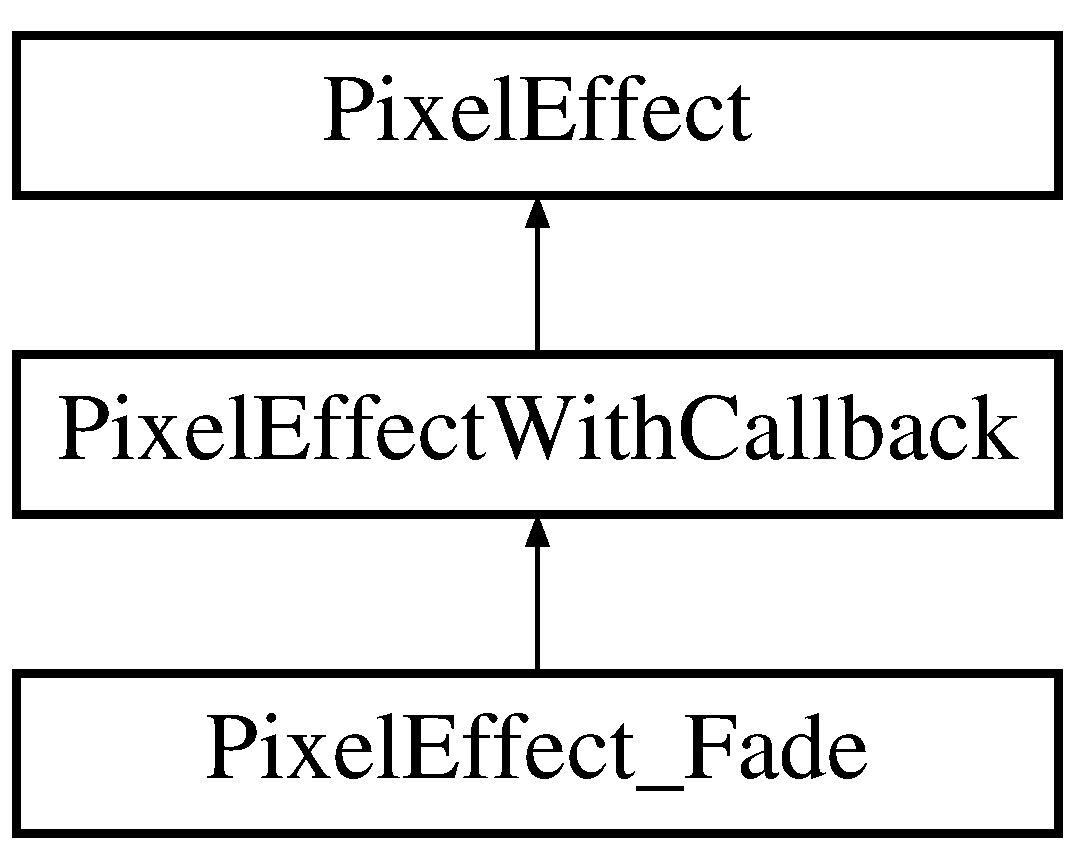
\includegraphics[height=3.000000cm]{class_pixel_effect___fade}
\end{center}
\end{figure}
\subsection*{Public Member Functions}
\begin{DoxyCompactItemize}
\item 
{\bf Pixel\+Effect\+\_\+\+Fade} ({\bf Pixel\+Strip} $\ast$strip, uint32\+\_\+t delay)
\item 
void {\bf init} ()
\item 
void {\bf run} ()
\end{DoxyCompactItemize}
\subsection*{Additional Inherited Members}


\subsection{Detailed Description}
This class fades the current display. The cb\+Finished will be called when this effect is complete 

\subsection{Constructor \& Destructor Documentation}
\index{Pixel\+Effect\+\_\+\+Fade@{Pixel\+Effect\+\_\+\+Fade}!Pixel\+Effect\+\_\+\+Fade@{Pixel\+Effect\+\_\+\+Fade}}
\index{Pixel\+Effect\+\_\+\+Fade@{Pixel\+Effect\+\_\+\+Fade}!Pixel\+Effect\+\_\+\+Fade@{Pixel\+Effect\+\_\+\+Fade}}
\subsubsection[{Pixel\+Effect\+\_\+\+Fade}]{\setlength{\rightskip}{0pt plus 5cm}Pixel\+Effect\+\_\+\+Fade\+::\+Pixel\+Effect\+\_\+\+Fade (
\begin{DoxyParamCaption}
\item[{{\bf Pixel\+Strip} $\ast$}]{strip, }
\item[{uint32\+\_\+t}]{delay}
\end{DoxyParamCaption}
)\hspace{0.3cm}{\ttfamily [inline]}}\label{class_pixel_effect___fade_a3564d110cfa327be3e65455b0feb6f84}
Create a fader using delay between steps 
\begin{DoxyParams}{Parameters}
{\em strip} & Physical strip or logical Panel pointer \\
\hline
{\em delay} & Delay between each fade step \\
\hline
\end{DoxyParams}


\subsection{Member Function Documentation}
\index{Pixel\+Effect\+\_\+\+Fade@{Pixel\+Effect\+\_\+\+Fade}!init@{init}}
\index{init@{init}!Pixel\+Effect\+\_\+\+Fade@{Pixel\+Effect\+\_\+\+Fade}}
\subsubsection[{init}]{\setlength{\rightskip}{0pt plus 5cm}void Pixel\+Effect\+\_\+\+Fade\+::init (
\begin{DoxyParamCaption}
{}
\end{DoxyParamCaption}
)\hspace{0.3cm}{\ttfamily [inline]}, {\ttfamily [virtual]}}\label{class_pixel_effect___fade_a4a9ec0355f7afec0967d446a0b70a4d5}
The init function, which must be called before the effect is \doxyref{run()}{p.}{class_pixel_effect___fade_ad538d7242223524b00c39104e2bc5001} 

Implements {\bf Pixel\+Effect} \doxyref{}{p.}{class_pixel_effect_ab3c11ba2c2f1cd26e62a0a8f16c6c02b}.

\index{Pixel\+Effect\+\_\+\+Fade@{Pixel\+Effect\+\_\+\+Fade}!run@{run}}
\index{run@{run}!Pixel\+Effect\+\_\+\+Fade@{Pixel\+Effect\+\_\+\+Fade}}
\subsubsection[{run}]{\setlength{\rightskip}{0pt plus 5cm}void Pixel\+Effect\+\_\+\+Fade\+::run (
\begin{DoxyParamCaption}
{}
\end{DoxyParamCaption}
)\hspace{0.3cm}{\ttfamily [inline]}, {\ttfamily [virtual]}}\label{class_pixel_effect___fade_ad538d7242223524b00c39104e2bc5001}
The \doxyref{run()}{p.}{class_pixel_effect___fade_ad538d7242223524b00c39104e2bc5001} function, which is called to update the state of the light effect 

Implements {\bf Pixel\+Effect} \doxyref{}{p.}{class_pixel_effect_adfff257c93348ebca93bcc7f38eee20d}.



The documentation for this class was generated from the following file\+:\begin{DoxyCompactItemize}
\item 
C\+:/\+Users/\+Russell/\+Documents/\+Arduino/libraries/\+Opcom\+\_\+\+Neo\+Pixel/Pixel\+Effect\+\_\+\+Fade.\+h\end{DoxyCompactItemize}

\section{Pixel\+Effect\+\_\+\+Fire Class Reference}
\label{class_pixel_effect___fire}\index{Pixel\+Effect\+\_\+\+Fire@{Pixel\+Effect\+\_\+\+Fire}}


{\ttfamily \#include $<$Pixel\+Effect\+\_\+\+Fire.\+h$>$}

Inheritance diagram for Pixel\+Effect\+\_\+\+Fire\+:\begin{figure}[H]
\begin{center}
\leavevmode
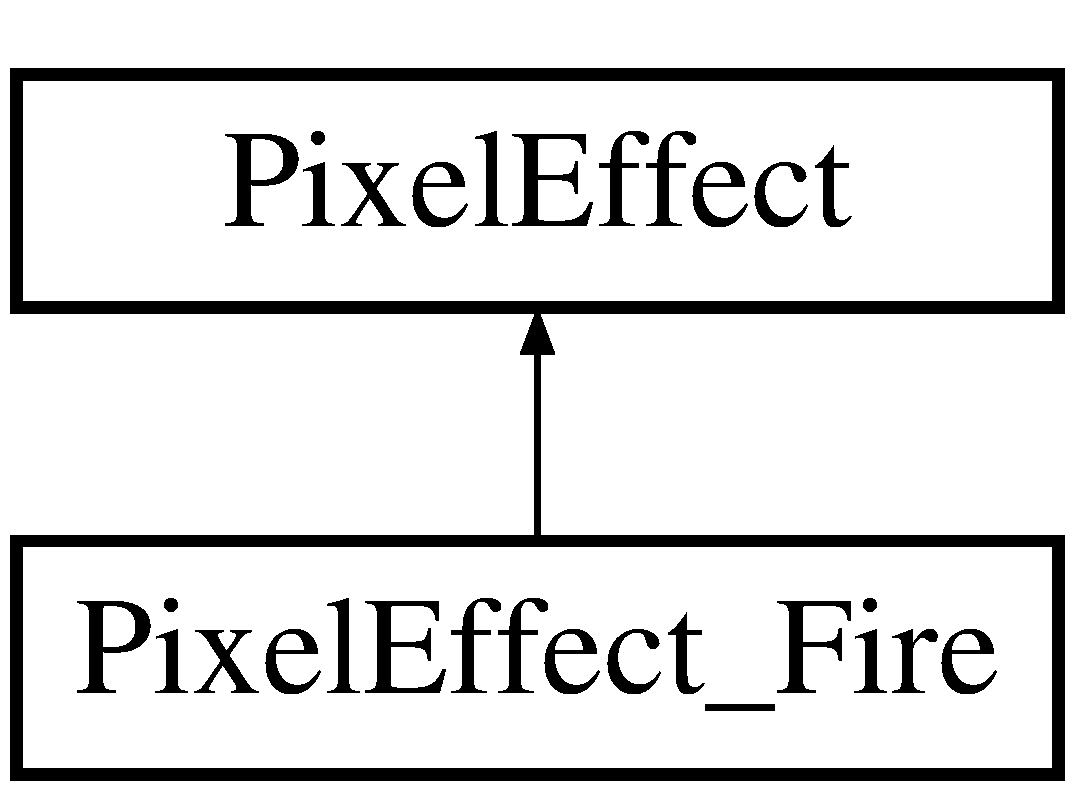
\includegraphics[height=2.000000cm]{class_pixel_effect___fire}
\end{center}
\end{figure}
\subsection*{Public Member Functions}
\begin{DoxyCompactItemize}
\item 
{\bf Pixel\+Effect\+\_\+\+Fire} ({\bf Pixel\+Strip} $\ast$strip)
\item 
void {\bf set\+Base\+Colors} (uint8\+\_\+t r, uint8\+\_\+t g, uint8\+\_\+t b)
\item 
void {\bf init} ()
\item 
void {\bf run} ()
\end{DoxyCompactItemize}
\subsection*{Additional Inherited Members}


\subsection{Detailed Description}
A display that looks like fire 

\subsection{Constructor \& Destructor Documentation}
\index{Pixel\+Effect\+\_\+\+Fire@{Pixel\+Effect\+\_\+\+Fire}!Pixel\+Effect\+\_\+\+Fire@{Pixel\+Effect\+\_\+\+Fire}}
\index{Pixel\+Effect\+\_\+\+Fire@{Pixel\+Effect\+\_\+\+Fire}!Pixel\+Effect\+\_\+\+Fire@{Pixel\+Effect\+\_\+\+Fire}}
\subsubsection[{Pixel\+Effect\+\_\+\+Fire}]{\setlength{\rightskip}{0pt plus 5cm}Pixel\+Effect\+\_\+\+Fire\+::\+Pixel\+Effect\+\_\+\+Fire (
\begin{DoxyParamCaption}
\item[{{\bf Pixel\+Strip} $\ast$}]{strip}
\end{DoxyParamCaption}
)\hspace{0.3cm}{\ttfamily [inline]}}\label{class_pixel_effect___fire_a71c2a0f0318b3233c23f4232a748bbda}
Create a fader using delay between steps 
\begin{DoxyParams}{Parameters}
{\em strip} & Physical strip or logical Panel pointer \\
\hline
\end{DoxyParams}


\subsection{Member Function Documentation}
\index{Pixel\+Effect\+\_\+\+Fire@{Pixel\+Effect\+\_\+\+Fire}!init@{init}}
\index{init@{init}!Pixel\+Effect\+\_\+\+Fire@{Pixel\+Effect\+\_\+\+Fire}}
\subsubsection[{init}]{\setlength{\rightskip}{0pt plus 5cm}void Pixel\+Effect\+\_\+\+Fire\+::init (
\begin{DoxyParamCaption}
{}
\end{DoxyParamCaption}
)\hspace{0.3cm}{\ttfamily [inline]}, {\ttfamily [virtual]}}\label{class_pixel_effect___fire_a210a5c79036f523f1a98fbf97a975d16}
The init function, which must be called before the effect is \doxyref{run()}{p.}{class_pixel_effect___fire_ac3d39af015e7005f8e345cc4d83d81f0} 

Implements {\bf Pixel\+Effect} \doxyref{}{p.}{class_pixel_effect_ab3c11ba2c2f1cd26e62a0a8f16c6c02b}.

\index{Pixel\+Effect\+\_\+\+Fire@{Pixel\+Effect\+\_\+\+Fire}!run@{run}}
\index{run@{run}!Pixel\+Effect\+\_\+\+Fire@{Pixel\+Effect\+\_\+\+Fire}}
\subsubsection[{run}]{\setlength{\rightskip}{0pt plus 5cm}void Pixel\+Effect\+\_\+\+Fire\+::run (
\begin{DoxyParamCaption}
{}
\end{DoxyParamCaption}
)\hspace{0.3cm}{\ttfamily [inline]}, {\ttfamily [virtual]}}\label{class_pixel_effect___fire_ac3d39af015e7005f8e345cc4d83d81f0}
The \doxyref{run()}{p.}{class_pixel_effect___fire_ac3d39af015e7005f8e345cc4d83d81f0} function, which is called to update the state of the light effect 

Implements {\bf Pixel\+Effect} \doxyref{}{p.}{class_pixel_effect_adfff257c93348ebca93bcc7f38eee20d}.

\index{Pixel\+Effect\+\_\+\+Fire@{Pixel\+Effect\+\_\+\+Fire}!set\+Base\+Colors@{set\+Base\+Colors}}
\index{set\+Base\+Colors@{set\+Base\+Colors}!Pixel\+Effect\+\_\+\+Fire@{Pixel\+Effect\+\_\+\+Fire}}
\subsubsection[{set\+Base\+Colors}]{\setlength{\rightskip}{0pt plus 5cm}void Pixel\+Effect\+\_\+\+Fire\+::set\+Base\+Colors (
\begin{DoxyParamCaption}
\item[{uint8\+\_\+t}]{r, }
\item[{uint8\+\_\+t}]{g, }
\item[{uint8\+\_\+t}]{b}
\end{DoxyParamCaption}
)\hspace{0.3cm}{\ttfamily [inline]}}\label{class_pixel_effect___fire_a82280bddb0a05efee7e56e8b88e298a7}
Set the base values for the colors to flicker. 
\begin{DoxyParams}{Parameters}
{\em r} & Red \\
\hline
{\em g} & Green \\
\hline
{\em b} & Blue \\
\hline
\end{DoxyParams}


The documentation for this class was generated from the following file\+:\begin{DoxyCompactItemize}
\item 
C\+:/\+Users/\+Russell/\+Documents/\+Arduino/libraries/\+Opcom\+\_\+\+Neo\+Pixel/Pixel\+Effect\+\_\+\+Fire.\+h\end{DoxyCompactItemize}

\section{Pixel\+Effect\+\_\+\+Flash Class Reference}
\label{class_pixel_effect___flash}\index{Pixel\+Effect\+\_\+\+Flash@{Pixel\+Effect\+\_\+\+Flash}}


{\ttfamily \#include $<$Pixel\+Effect\+\_\+\+Flash.\+h$>$}

Inheritance diagram for Pixel\+Effect\+\_\+\+Flash\+:\begin{figure}[H]
\begin{center}
\leavevmode
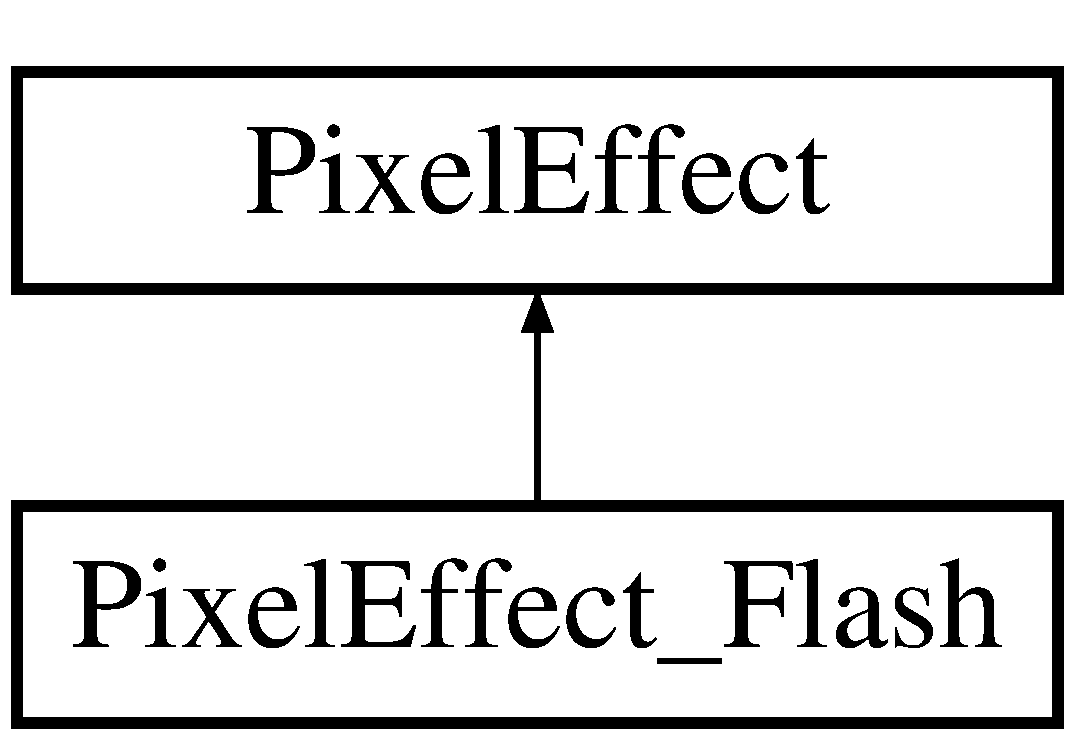
\includegraphics[height=2.000000cm]{class_pixel_effect___flash}
\end{center}
\end{figure}
\subsection*{Public Member Functions}
\begin{DoxyCompactItemize}
\item 
{\bf Pixel\+Effect\+\_\+\+Flash} ({\bf Pixel\+Strip} $\ast$strip, uint32\+\_\+t color\+On, uint32\+\_\+t on\+Time, uint32\+\_\+t color\+Off, uint32\+\_\+t off\+Time)
\item 
void {\bf init} ()
\item 
void {\bf run} ()
\end{DoxyCompactItemize}
\subsection*{Additional Inherited Members}


\subsection{Detailed Description}
Flashes a color on and off, with configurable on and off time 

\subsection{Constructor \& Destructor Documentation}
\index{Pixel\+Effect\+\_\+\+Flash@{Pixel\+Effect\+\_\+\+Flash}!Pixel\+Effect\+\_\+\+Flash@{Pixel\+Effect\+\_\+\+Flash}}
\index{Pixel\+Effect\+\_\+\+Flash@{Pixel\+Effect\+\_\+\+Flash}!Pixel\+Effect\+\_\+\+Flash@{Pixel\+Effect\+\_\+\+Flash}}
\subsubsection[{Pixel\+Effect\+\_\+\+Flash}]{\setlength{\rightskip}{0pt plus 5cm}Pixel\+Effect\+\_\+\+Flash\+::\+Pixel\+Effect\+\_\+\+Flash (
\begin{DoxyParamCaption}
\item[{{\bf Pixel\+Strip} $\ast$}]{strip, }
\item[{uint32\+\_\+t}]{color\+On, }
\item[{uint32\+\_\+t}]{on\+Time, }
\item[{uint32\+\_\+t}]{color\+Off, }
\item[{uint32\+\_\+t}]{off\+Time}
\end{DoxyParamCaption}
)\hspace{0.3cm}{\ttfamily [inline]}}\label{class_pixel_effect___flash_a4033d8ba5e3ac05315e3b5cda3277ebd}
Flash a color on and off. 
\begin{DoxyParams}{Parameters}
{\em strip} & Physical strip or logical Panel pointer \\
\hline
{\em color\+On} & Color to flash \\
\hline
{\em on\+Time} & milliseconds for on state \\
\hline
{\em color\+Off} & Color during \textquotesingle{}off\textquotesingle{} state \\
\hline
{\em off\+Time} & milliseconds for off state \\
\hline
\end{DoxyParams}


\subsection{Member Function Documentation}
\index{Pixel\+Effect\+\_\+\+Flash@{Pixel\+Effect\+\_\+\+Flash}!init@{init}}
\index{init@{init}!Pixel\+Effect\+\_\+\+Flash@{Pixel\+Effect\+\_\+\+Flash}}
\subsubsection[{init}]{\setlength{\rightskip}{0pt plus 5cm}void Pixel\+Effect\+\_\+\+Flash\+::init (
\begin{DoxyParamCaption}
{}
\end{DoxyParamCaption}
)\hspace{0.3cm}{\ttfamily [inline]}, {\ttfamily [virtual]}}\label{class_pixel_effect___flash_a4563d09b05c4af920675f7246d136c27}
The init function, which must be called before the effect is \doxyref{run()}{p.}{class_pixel_effect___flash_a96a43629b9422fc10420ab48604e08e2} 

Implements {\bf Pixel\+Effect} \doxyref{}{p.}{class_pixel_effect_ab3c11ba2c2f1cd26e62a0a8f16c6c02b}.

\index{Pixel\+Effect\+\_\+\+Flash@{Pixel\+Effect\+\_\+\+Flash}!run@{run}}
\index{run@{run}!Pixel\+Effect\+\_\+\+Flash@{Pixel\+Effect\+\_\+\+Flash}}
\subsubsection[{run}]{\setlength{\rightskip}{0pt plus 5cm}void Pixel\+Effect\+\_\+\+Flash\+::run (
\begin{DoxyParamCaption}
{}
\end{DoxyParamCaption}
)\hspace{0.3cm}{\ttfamily [inline]}, {\ttfamily [virtual]}}\label{class_pixel_effect___flash_a96a43629b9422fc10420ab48604e08e2}
The \doxyref{run()}{p.}{class_pixel_effect___flash_a96a43629b9422fc10420ab48604e08e2} function, which is called to update the state of the light effect 

Implements {\bf Pixel\+Effect} \doxyref{}{p.}{class_pixel_effect_adfff257c93348ebca93bcc7f38eee20d}.



The documentation for this class was generated from the following file\+:\begin{DoxyCompactItemize}
\item 
C\+:/\+Users/\+Russell/\+Documents/\+Arduino/libraries/\+Opcom\+\_\+\+Neo\+Pixel/Pixel\+Effect\+\_\+\+Flash.\+h\end{DoxyCompactItemize}

\section{Pixel\+Effect\+\_\+\+Knight\+Rider Class Reference}
\label{class_pixel_effect___knight_rider}\index{Pixel\+Effect\+\_\+\+Knight\+Rider@{Pixel\+Effect\+\_\+\+Knight\+Rider}}


{\ttfamily \#include $<$Pixel\+Effect\+\_\+\+Night\+Rider.\+h$>$}

Inheritance diagram for Pixel\+Effect\+\_\+\+Knight\+Rider\+:\begin{figure}[H]
\begin{center}
\leavevmode
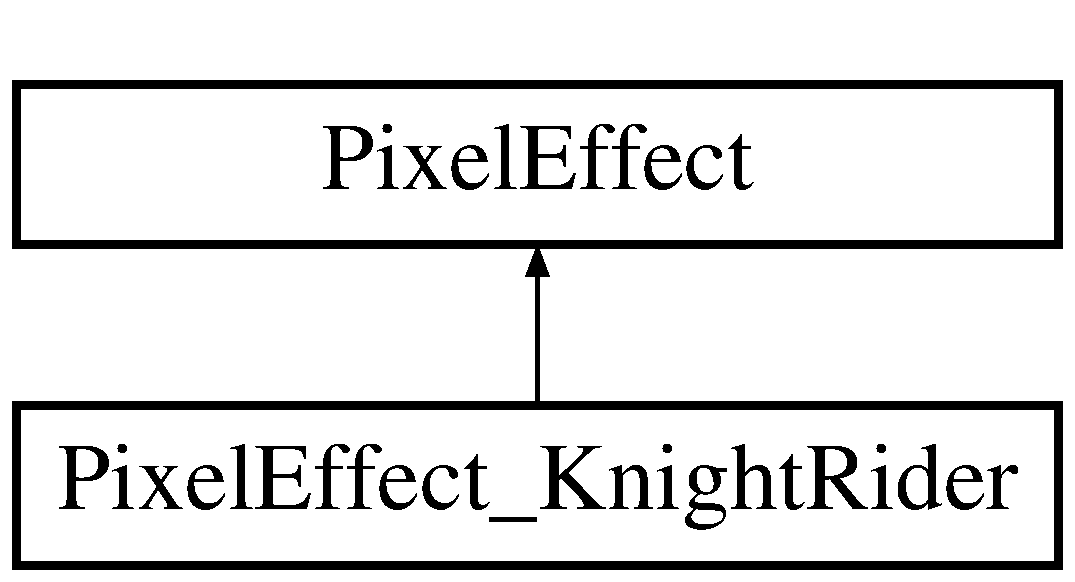
\includegraphics[height=2.000000cm]{class_pixel_effect___knight_rider}
\end{center}
\end{figure}
\subsection*{Public Member Functions}
\begin{DoxyCompactItemize}
\item 
{\bf Pixel\+Effect\+\_\+\+Knight\+Rider} ({\bf Pixel\+Strip} $\ast$strip, uint16\+\_\+t speed=32, uint8\+\_\+t width=4, uint32\+\_\+t color=0x\+F\+F1000)
\item 
void {\bf init} ()
\item 
void {\bf run} ()
\end{DoxyCompactItemize}
\subsection*{Additional Inherited Members}


\subsection{Detailed Description}
A Kinght Rider effect of pixels moving back and forth across the panel 

\subsection{Constructor \& Destructor Documentation}
\index{Pixel\+Effect\+\_\+\+Knight\+Rider@{Pixel\+Effect\+\_\+\+Knight\+Rider}!Pixel\+Effect\+\_\+\+Knight\+Rider@{Pixel\+Effect\+\_\+\+Knight\+Rider}}
\index{Pixel\+Effect\+\_\+\+Knight\+Rider@{Pixel\+Effect\+\_\+\+Knight\+Rider}!Pixel\+Effect\+\_\+\+Knight\+Rider@{Pixel\+Effect\+\_\+\+Knight\+Rider}}
\subsubsection[{Pixel\+Effect\+\_\+\+Knight\+Rider}]{\setlength{\rightskip}{0pt plus 5cm}Pixel\+Effect\+\_\+\+Knight\+Rider\+::\+Pixel\+Effect\+\_\+\+Knight\+Rider (
\begin{DoxyParamCaption}
\item[{{\bf Pixel\+Strip} $\ast$}]{strip, }
\item[{uint16\+\_\+t}]{speed = {\ttfamily 32}, }
\item[{uint8\+\_\+t}]{width = {\ttfamily 4}, }
\item[{uint32\+\_\+t}]{color = {\ttfamily 0xFF1000}}
\end{DoxyParamCaption}
)\hspace{0.3cm}{\ttfamily [inline]}}\label{class_pixel_effect___knight_rider_a7bcca4f679f214d9f5d4d3361237fa99}
Does a display like the car Kit in the Knight Rider T\+V show 
\begin{DoxyParams}{Parameters}
{\em strip} & Physical strip or logical Panel pointer \\
\hline
{\em speed} & how fast one cycle is (32 with 16 pixels is default Knight\+Rider speed) \\
\hline
{\em width} & how wide the trail effect is on the fading out L\+E\+Ds. The original display used light bulbs, so they have a persistance when turning off. This creates a trail. Effective range is 2 -\/ 8, 4 is default for 16 pixels. Play with this. \\
\hline
{\em color} & 32-\/bit packed R\+G\+B color value. Defaults to T\+V series color \\
\hline
\end{DoxyParams}


\subsection{Member Function Documentation}
\index{Pixel\+Effect\+\_\+\+Knight\+Rider@{Pixel\+Effect\+\_\+\+Knight\+Rider}!init@{init}}
\index{init@{init}!Pixel\+Effect\+\_\+\+Knight\+Rider@{Pixel\+Effect\+\_\+\+Knight\+Rider}}
\subsubsection[{init}]{\setlength{\rightskip}{0pt plus 5cm}void Pixel\+Effect\+\_\+\+Knight\+Rider\+::init (
\begin{DoxyParamCaption}
{}
\end{DoxyParamCaption}
)\hspace{0.3cm}{\ttfamily [inline]}, {\ttfamily [virtual]}}\label{class_pixel_effect___knight_rider_a16b3569280331671f795e367b4f4dd54}
The init function, which must be called before the effect is \doxyref{run()}{p.}{class_pixel_effect___knight_rider_a35c58ed5e875365942e4666d43eafe39} 

Implements {\bf Pixel\+Effect} \doxyref{}{p.}{class_pixel_effect_ab3c11ba2c2f1cd26e62a0a8f16c6c02b}.

\index{Pixel\+Effect\+\_\+\+Knight\+Rider@{Pixel\+Effect\+\_\+\+Knight\+Rider}!run@{run}}
\index{run@{run}!Pixel\+Effect\+\_\+\+Knight\+Rider@{Pixel\+Effect\+\_\+\+Knight\+Rider}}
\subsubsection[{run}]{\setlength{\rightskip}{0pt plus 5cm}void Pixel\+Effect\+\_\+\+Knight\+Rider\+::run (
\begin{DoxyParamCaption}
{}
\end{DoxyParamCaption}
)\hspace{0.3cm}{\ttfamily [inline]}, {\ttfamily [virtual]}}\label{class_pixel_effect___knight_rider_a35c58ed5e875365942e4666d43eafe39}
The \doxyref{run()}{p.}{class_pixel_effect___knight_rider_a35c58ed5e875365942e4666d43eafe39} function, which is called to update the state of the light effect 

Implements {\bf Pixel\+Effect} \doxyref{}{p.}{class_pixel_effect_adfff257c93348ebca93bcc7f38eee20d}.



The documentation for this class was generated from the following file\+:\begin{DoxyCompactItemize}
\item 
C\+:/\+Users/\+Russell/\+Documents/\+Arduino/libraries/\+Opcom\+\_\+\+Neo\+Pixel/Pixel\+Effect\+\_\+\+Night\+Rider.\+h\end{DoxyCompactItemize}

\section{Pixel\+Effect\+\_\+\+Solid Class Reference}
\label{class_pixel_effect___solid}\index{Pixel\+Effect\+\_\+\+Solid@{Pixel\+Effect\+\_\+\+Solid}}


{\ttfamily \#include $<$Pixel\+Effect\+\_\+\+Solid.\+h$>$}

Inheritance diagram for Pixel\+Effect\+\_\+\+Solid\+:\begin{figure}[H]
\begin{center}
\leavevmode
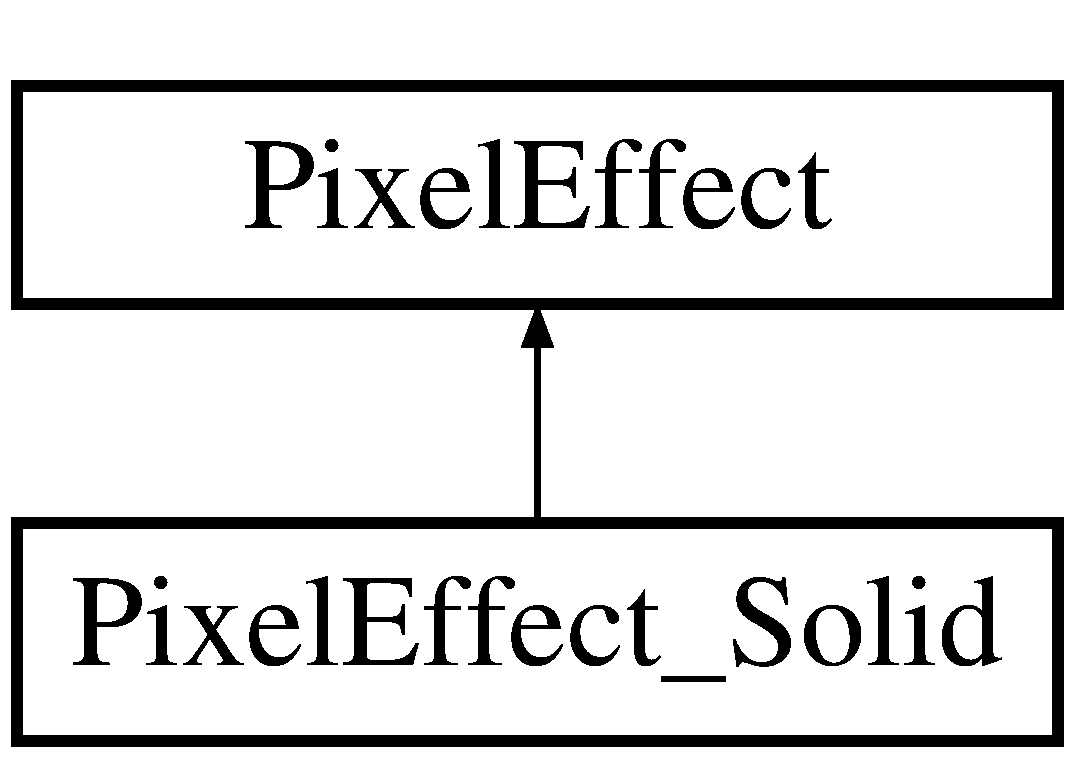
\includegraphics[height=2.000000cm]{class_pixel_effect___solid}
\end{center}
\end{figure}
\subsection*{Public Member Functions}
\begin{DoxyCompactItemize}
\item 
{\bf Pixel\+Effect\+\_\+\+Solid} ({\bf Pixel\+Strip} $\ast$strip, uint32\+\_\+t color)
\item 
void {\bf init} ()
\item 
void {\bf run} ()
\end{DoxyCompactItemize}
\subsection*{Protected Attributes}
\begin{DoxyCompactItemize}
\item 
uint32\+\_\+t {\bfseries m\+\_\+color}\label{class_pixel_effect___solid_ab4f2eb82c75660bf031b6c21e2b45fa7}

\end{DoxyCompactItemize}
\subsection*{Additional Inherited Members}


\subsection{Detailed Description}
Create a solid color that does not change. Every call to run will recreate the color, so in most cases, this effect can be \doxyref{run()}{p.}{class_pixel_effect___solid_a2a5887f47c4f56d23707387be85d5b6b} once then disabled, if no other display is running on the panel. 

\subsection{Constructor \& Destructor Documentation}
\index{Pixel\+Effect\+\_\+\+Solid@{Pixel\+Effect\+\_\+\+Solid}!Pixel\+Effect\+\_\+\+Solid@{Pixel\+Effect\+\_\+\+Solid}}
\index{Pixel\+Effect\+\_\+\+Solid@{Pixel\+Effect\+\_\+\+Solid}!Pixel\+Effect\+\_\+\+Solid@{Pixel\+Effect\+\_\+\+Solid}}
\subsubsection[{Pixel\+Effect\+\_\+\+Solid}]{\setlength{\rightskip}{0pt plus 5cm}Pixel\+Effect\+\_\+\+Solid\+::\+Pixel\+Effect\+\_\+\+Solid (
\begin{DoxyParamCaption}
\item[{{\bf Pixel\+Strip} $\ast$}]{strip, }
\item[{uint32\+\_\+t}]{color}
\end{DoxyParamCaption}
)\hspace{0.3cm}{\ttfamily [inline]}}\label{class_pixel_effect___solid_a93a5a69f9f3deaa0c62d05a2eec5f284}
Create a solid fill. 
\begin{DoxyParams}{Parameters}
{\em strip} & Physical strip or logical Panel pointer \\
\hline
{\em color} & Solid R\+G\+B color to display \\
\hline
\end{DoxyParams}


\subsection{Member Function Documentation}
\index{Pixel\+Effect\+\_\+\+Solid@{Pixel\+Effect\+\_\+\+Solid}!init@{init}}
\index{init@{init}!Pixel\+Effect\+\_\+\+Solid@{Pixel\+Effect\+\_\+\+Solid}}
\subsubsection[{init}]{\setlength{\rightskip}{0pt plus 5cm}void Pixel\+Effect\+\_\+\+Solid\+::init (
\begin{DoxyParamCaption}
{}
\end{DoxyParamCaption}
)\hspace{0.3cm}{\ttfamily [inline]}, {\ttfamily [virtual]}}\label{class_pixel_effect___solid_a74c03fc565fde97566240ea176b7b5ce}
The init function, which must be called before the effect is \doxyref{run()}{p.}{class_pixel_effect___solid_a2a5887f47c4f56d23707387be85d5b6b} 

Implements {\bf Pixel\+Effect} \doxyref{}{p.}{class_pixel_effect_ab3c11ba2c2f1cd26e62a0a8f16c6c02b}.

\index{Pixel\+Effect\+\_\+\+Solid@{Pixel\+Effect\+\_\+\+Solid}!run@{run}}
\index{run@{run}!Pixel\+Effect\+\_\+\+Solid@{Pixel\+Effect\+\_\+\+Solid}}
\subsubsection[{run}]{\setlength{\rightskip}{0pt plus 5cm}void Pixel\+Effect\+\_\+\+Solid\+::run (
\begin{DoxyParamCaption}
{}
\end{DoxyParamCaption}
)\hspace{0.3cm}{\ttfamily [inline]}, {\ttfamily [virtual]}}\label{class_pixel_effect___solid_a2a5887f47c4f56d23707387be85d5b6b}
The \doxyref{run()}{p.}{class_pixel_effect___solid_a2a5887f47c4f56d23707387be85d5b6b} function, which is called to update the state of the light effect 

Implements {\bf Pixel\+Effect} \doxyref{}{p.}{class_pixel_effect_adfff257c93348ebca93bcc7f38eee20d}.



The documentation for this class was generated from the following file\+:\begin{DoxyCompactItemize}
\item 
C\+:/\+Users/\+Russell/\+Documents/\+Arduino/libraries/\+Opcom\+\_\+\+Neo\+Pixel/Pixel\+Effect\+\_\+\+Solid.\+h\end{DoxyCompactItemize}

\section{Pixel\+Effect\+\_\+\+Theatre\+Chase Class Reference}
\label{class_pixel_effect___theatre_chase}\index{Pixel\+Effect\+\_\+\+Theatre\+Chase@{Pixel\+Effect\+\_\+\+Theatre\+Chase}}


{\ttfamily \#include $<$Pixel\+Effect\+\_\+\+Theatre\+Chase.\+h$>$}

Inheritance diagram for Pixel\+Effect\+\_\+\+Theatre\+Chase\+:\begin{figure}[H]
\begin{center}
\leavevmode
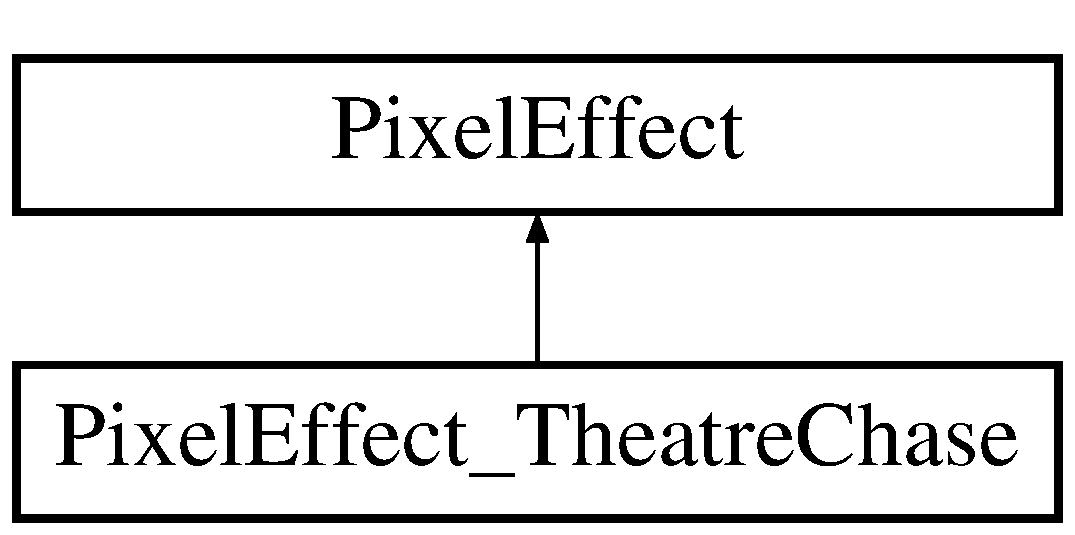
\includegraphics[height=2.000000cm]{class_pixel_effect___theatre_chase}
\end{center}
\end{figure}
\subsection*{Public Member Functions}
\begin{DoxyCompactItemize}
\item 
{\bf Pixel\+Effect\+\_\+\+Theatre\+Chase} ({\bf Pixel\+Strip} $\ast$strip, uint32\+\_\+t color, uint32\+\_\+t wait, bool reverse=false)
\item 
void {\bf init} ()
\item 
void {\bf run} ()
\end{DoxyCompactItemize}
\subsection*{Additional Inherited Members}


\subsection{Detailed Description}
Theatre-\/style crawling lights. 

\subsection{Constructor \& Destructor Documentation}
\index{Pixel\+Effect\+\_\+\+Theatre\+Chase@{Pixel\+Effect\+\_\+\+Theatre\+Chase}!Pixel\+Effect\+\_\+\+Theatre\+Chase@{Pixel\+Effect\+\_\+\+Theatre\+Chase}}
\index{Pixel\+Effect\+\_\+\+Theatre\+Chase@{Pixel\+Effect\+\_\+\+Theatre\+Chase}!Pixel\+Effect\+\_\+\+Theatre\+Chase@{Pixel\+Effect\+\_\+\+Theatre\+Chase}}
\subsubsection[{Pixel\+Effect\+\_\+\+Theatre\+Chase}]{\setlength{\rightskip}{0pt plus 5cm}Pixel\+Effect\+\_\+\+Theatre\+Chase\+::\+Pixel\+Effect\+\_\+\+Theatre\+Chase (
\begin{DoxyParamCaption}
\item[{{\bf Pixel\+Strip} $\ast$}]{strip, }
\item[{uint32\+\_\+t}]{color, }
\item[{uint32\+\_\+t}]{wait, }
\item[{bool}]{reverse = {\ttfamily false}}
\end{DoxyParamCaption}
)\hspace{0.3cm}{\ttfamily [inline]}}\label{class_pixel_effect___theatre_chase_a3616649acadefb4924662d7fa682b7dc}
Theatre-\/style crawling lights. 
\begin{DoxyParams}{Parameters}
{\em strip} & Physical strip or logical Panel pointer \\
\hline
{\em color} & The color to wipe \\
\hline
{\em wait} & Milliseconds to wait between transitions \\
\hline
{\em reverse} & Reverses crawl direction \\
\hline
\end{DoxyParams}


\subsection{Member Function Documentation}
\index{Pixel\+Effect\+\_\+\+Theatre\+Chase@{Pixel\+Effect\+\_\+\+Theatre\+Chase}!init@{init}}
\index{init@{init}!Pixel\+Effect\+\_\+\+Theatre\+Chase@{Pixel\+Effect\+\_\+\+Theatre\+Chase}}
\subsubsection[{init}]{\setlength{\rightskip}{0pt plus 5cm}void Pixel\+Effect\+\_\+\+Theatre\+Chase\+::init (
\begin{DoxyParamCaption}
{}
\end{DoxyParamCaption}
)\hspace{0.3cm}{\ttfamily [inline]}, {\ttfamily [virtual]}}\label{class_pixel_effect___theatre_chase_a6576f90406a69407d9b6633b30e1075e}
The init function, which must be called before the effect is \doxyref{run()}{p.}{class_pixel_effect___theatre_chase_a18283d29998b59918d604893cd3e9527} 

Implements {\bf Pixel\+Effect} \doxyref{}{p.}{class_pixel_effect_ab3c11ba2c2f1cd26e62a0a8f16c6c02b}.

\index{Pixel\+Effect\+\_\+\+Theatre\+Chase@{Pixel\+Effect\+\_\+\+Theatre\+Chase}!run@{run}}
\index{run@{run}!Pixel\+Effect\+\_\+\+Theatre\+Chase@{Pixel\+Effect\+\_\+\+Theatre\+Chase}}
\subsubsection[{run}]{\setlength{\rightskip}{0pt plus 5cm}void Pixel\+Effect\+\_\+\+Theatre\+Chase\+::run (
\begin{DoxyParamCaption}
{}
\end{DoxyParamCaption}
)\hspace{0.3cm}{\ttfamily [inline]}, {\ttfamily [virtual]}}\label{class_pixel_effect___theatre_chase_a18283d29998b59918d604893cd3e9527}
The \doxyref{run()}{p.}{class_pixel_effect___theatre_chase_a18283d29998b59918d604893cd3e9527} function, which is called to update the state of the light effect 

Implements {\bf Pixel\+Effect} \doxyref{}{p.}{class_pixel_effect_adfff257c93348ebca93bcc7f38eee20d}.



The documentation for this class was generated from the following file\+:\begin{DoxyCompactItemize}
\item 
C\+:/\+Users/\+Russell/\+Documents/\+Arduino/libraries/\+Opcom\+\_\+\+Neo\+Pixel/Pixel\+Effect\+\_\+\+Theatre\+Chase.\+h\end{DoxyCompactItemize}

\section{Pixel\+Effect\+Stack Class Reference}
\label{class_pixel_effect_stack}\index{Pixel\+Effect\+Stack@{Pixel\+Effect\+Stack}}


{\ttfamily \#include $<$Pixel\+Effect\+Stack.\+h$>$}

Inheritance diagram for Pixel\+Effect\+Stack\+:\begin{figure}[H]
\begin{center}
\leavevmode
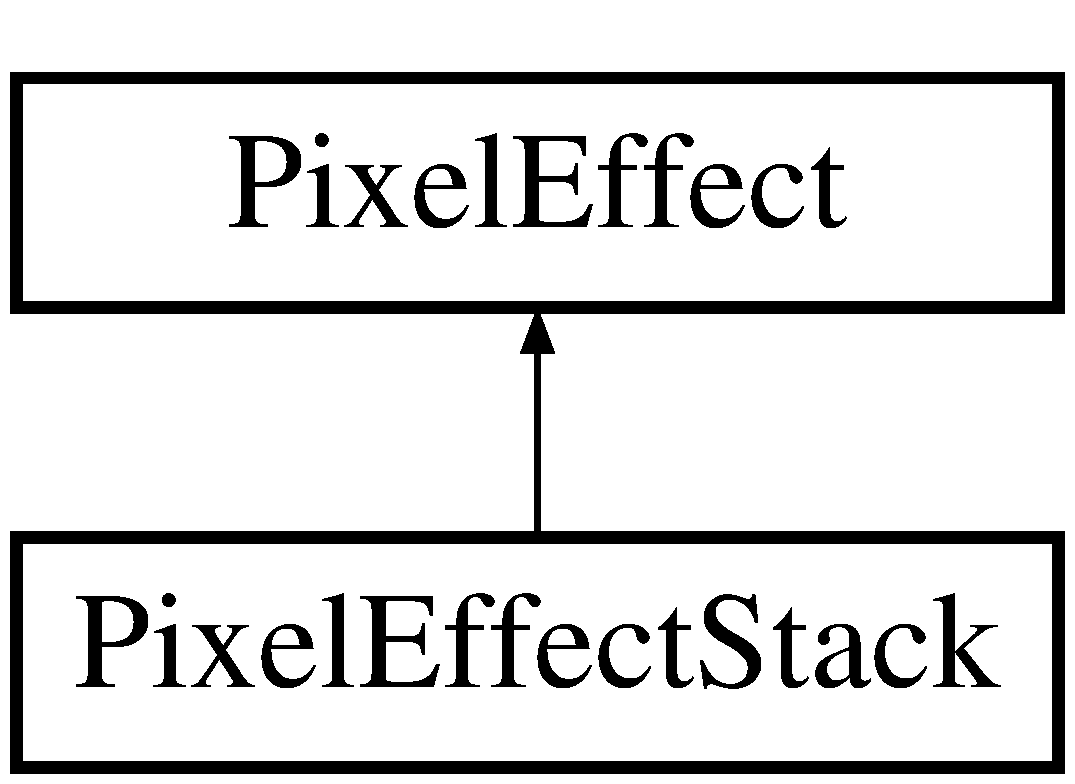
\includegraphics[height=2.000000cm]{class_pixel_effect_stack}
\end{center}
\end{figure}
\subsection*{Public Member Functions}
\begin{DoxyCompactItemize}
\item 
{\bf Pixel\+Effect\+Stack} ({\bf Pixel\+Strip} $\ast$strip=N\+U\+L\+L)
\item 
void {\bf add\+Effect} ({\bf Pixel\+Effect} $\ast$pe)
\item 
void {\bf init} ()
\item 
void {\bf run} ()
\end{DoxyCompactItemize}
\subsection*{Additional Inherited Members}


\subsection{Detailed Description}
This is not currently implemented. Stack effects in a panel on top of each other, so that one draws on top of another. \begin{DoxyRefDesc}{Todo}
\item[{\bf Todo}]Debug arduino to find out why only a few pixels are displayed when using the Knight Rider effect. See code in comments \end{DoxyRefDesc}


\subsection{Constructor \& Destructor Documentation}
\index{Pixel\+Effect\+Stack@{Pixel\+Effect\+Stack}!Pixel\+Effect\+Stack@{Pixel\+Effect\+Stack}}
\index{Pixel\+Effect\+Stack@{Pixel\+Effect\+Stack}!Pixel\+Effect\+Stack@{Pixel\+Effect\+Stack}}
\subsubsection[{Pixel\+Effect\+Stack}]{\setlength{\rightskip}{0pt plus 5cm}Pixel\+Effect\+Stack\+::\+Pixel\+Effect\+Stack (
\begin{DoxyParamCaption}
\item[{{\bf Pixel\+Strip} $\ast$}]{strip = {\ttfamily NULL}}
\end{DoxyParamCaption}
)\hspace{0.3cm}{\ttfamily [inline]}}\label{class_pixel_effect_stack_ae03b1bff6950782c5e6f94c388bf44a9}
Create an effect stack for a strip 
\begin{DoxyParams}{Parameters}
{\em strip} & Physical strip or logical Panel pointer \\
\hline
\end{DoxyParams}


\subsection{Member Function Documentation}
\index{Pixel\+Effect\+Stack@{Pixel\+Effect\+Stack}!add\+Effect@{add\+Effect}}
\index{add\+Effect@{add\+Effect}!Pixel\+Effect\+Stack@{Pixel\+Effect\+Stack}}
\subsubsection[{add\+Effect}]{\setlength{\rightskip}{0pt plus 5cm}void Pixel\+Effect\+Stack\+::add\+Effect (
\begin{DoxyParamCaption}
\item[{{\bf Pixel\+Effect} $\ast$}]{pe}
\end{DoxyParamCaption}
)\hspace{0.3cm}{\ttfamily [inline]}}\label{class_pixel_effect_stack_a5fff09c7f64a63b7e0a68e33d3a0abbf}
Add an effect to the stack. The last effect added is run last, so it will draw on top of any earlier effects. Create Pixel\+Effects with new() as this class will take ownership of the pe pointer. 
\begin{DoxyParams}{Parameters}
{\em pe} & A \doxyref{Pixel\+Effect}{p.}{class_pixel_effect} pointer. Warning... these will be free()d by this class on destruction. \\
\hline
\end{DoxyParams}
\index{Pixel\+Effect\+Stack@{Pixel\+Effect\+Stack}!init@{init}}
\index{init@{init}!Pixel\+Effect\+Stack@{Pixel\+Effect\+Stack}}
\subsubsection[{init}]{\setlength{\rightskip}{0pt plus 5cm}void Pixel\+Effect\+Stack\+::init (
\begin{DoxyParamCaption}
{}
\end{DoxyParamCaption}
)\hspace{0.3cm}{\ttfamily [inline]}, {\ttfamily [virtual]}}\label{class_pixel_effect_stack_a726083b8f63898358945226fa175757b}
The init function, which must be called before the effect is \doxyref{run()}{p.}{class_pixel_effect_stack_a6fbd31bab015a7d3526915a60392cbd1} 

Implements {\bf Pixel\+Effect} \doxyref{}{p.}{class_pixel_effect_ab3c11ba2c2f1cd26e62a0a8f16c6c02b}.

\index{Pixel\+Effect\+Stack@{Pixel\+Effect\+Stack}!run@{run}}
\index{run@{run}!Pixel\+Effect\+Stack@{Pixel\+Effect\+Stack}}
\subsubsection[{run}]{\setlength{\rightskip}{0pt plus 5cm}void Pixel\+Effect\+Stack\+::run (
\begin{DoxyParamCaption}
{}
\end{DoxyParamCaption}
)\hspace{0.3cm}{\ttfamily [inline]}, {\ttfamily [virtual]}}\label{class_pixel_effect_stack_a6fbd31bab015a7d3526915a60392cbd1}
The \doxyref{run()}{p.}{class_pixel_effect_stack_a6fbd31bab015a7d3526915a60392cbd1} function, which is called to update the state of the light effect 

Implements {\bf Pixel\+Effect} \doxyref{}{p.}{class_pixel_effect_adfff257c93348ebca93bcc7f38eee20d}.



The documentation for this class was generated from the following file\+:\begin{DoxyCompactItemize}
\item 
C\+:/\+Users/\+Russell/\+Documents/\+Arduino/libraries/\+Opcom\+\_\+\+Neo\+Pixel/Pixel\+Effect\+Stack.\+h\end{DoxyCompactItemize}

\section{Pixel\+Effect\+With\+Callback Class Reference}
\label{class_pixel_effect_with_callback}\index{Pixel\+Effect\+With\+Callback@{Pixel\+Effect\+With\+Callback}}


{\ttfamily \#include $<$Pixel\+Effect\+With\+Callback.\+h$>$}

Inheritance diagram for Pixel\+Effect\+With\+Callback\+:\begin{figure}[H]
\begin{center}
\leavevmode
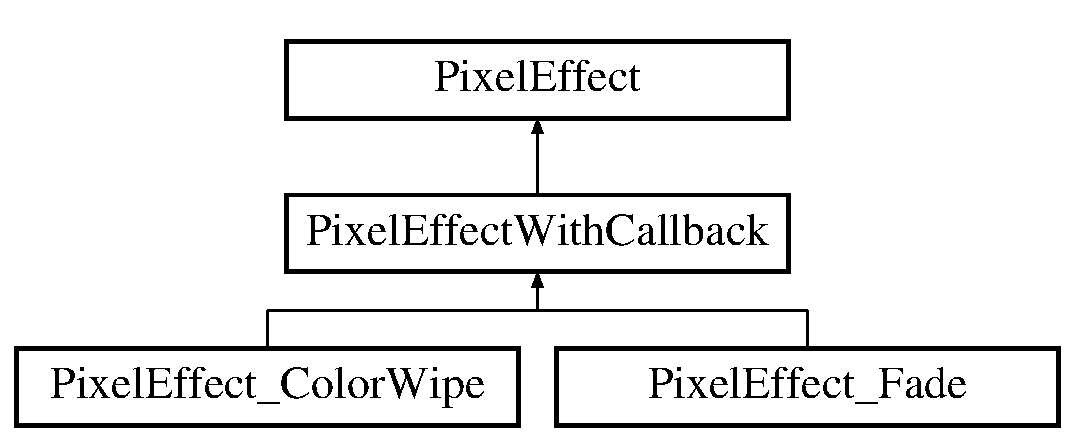
\includegraphics[height=3.000000cm]{class_pixel_effect_with_callback}
\end{center}
\end{figure}
\subsection*{Public Attributes}
\begin{DoxyCompactItemize}
\item 
volatile effect\+Callback {\bf cb\+Init}
\item 
volatile effect\+Callback {\bf cb\+One}
\item 
volatile effect\+Callback {\bf cb\+Two}
\item 
volatile effect\+Callback {\bf cb\+Three}
\item 
volatile effect\+Callback {\bf cb\+Four}
\item 
volatile effect\+Callback {\bf cb\+Finished}
\end{DoxyCompactItemize}
\subsection*{Protected Member Functions}
\begin{DoxyCompactItemize}
\item 
{\bf Pixel\+Effect\+With\+Callback} ({\bf Pixel\+Strip} $\ast$strip)
\end{DoxyCompactItemize}
\subsection*{Additional Inherited Members}


\subsection{Detailed Description}
Pixel effects that can fire callback events to handler functions. The use of the various callbacks is entirely up to the effect itself, so check the documentation of the effect. 

\subsection{Constructor \& Destructor Documentation}
\index{Pixel\+Effect\+With\+Callback@{Pixel\+Effect\+With\+Callback}!Pixel\+Effect\+With\+Callback@{Pixel\+Effect\+With\+Callback}}
\index{Pixel\+Effect\+With\+Callback@{Pixel\+Effect\+With\+Callback}!Pixel\+Effect\+With\+Callback@{Pixel\+Effect\+With\+Callback}}
\subsubsection[{Pixel\+Effect\+With\+Callback}]{\setlength{\rightskip}{0pt plus 5cm}Pixel\+Effect\+With\+Callback\+::\+Pixel\+Effect\+With\+Callback (
\begin{DoxyParamCaption}
\item[{{\bf Pixel\+Strip} $\ast$}]{strip}
\end{DoxyParamCaption}
)\hspace{0.3cm}{\ttfamily [inline]}, {\ttfamily [protected]}}\label{class_pixel_effect_with_callback_afd0d80cddf0c3c7d412baf0cae6a0d22}
Base constructor 

\subsection{Member Data Documentation}
\index{Pixel\+Effect\+With\+Callback@{Pixel\+Effect\+With\+Callback}!cb\+Finished@{cb\+Finished}}
\index{cb\+Finished@{cb\+Finished}!Pixel\+Effect\+With\+Callback@{Pixel\+Effect\+With\+Callback}}
\subsubsection[{cb\+Finished}]{\setlength{\rightskip}{0pt plus 5cm}volatile effect\+Callback Pixel\+Effect\+With\+Callback\+::cb\+Finished}\label{class_pixel_effect_with_callback_ab85c5f65ce18e18314c516fc960e5d1c}
Generally called if an effect actually has a \textquotesingle{}finished\textquotesingle{} state \index{Pixel\+Effect\+With\+Callback@{Pixel\+Effect\+With\+Callback}!cb\+Four@{cb\+Four}}
\index{cb\+Four@{cb\+Four}!Pixel\+Effect\+With\+Callback@{Pixel\+Effect\+With\+Callback}}
\subsubsection[{cb\+Four}]{\setlength{\rightskip}{0pt plus 5cm}volatile effect\+Callback Pixel\+Effect\+With\+Callback\+::cb\+Four}\label{class_pixel_effect_with_callback_af4cb7aabda135c035b1b22be904a9b31}
Callback slot \index{Pixel\+Effect\+With\+Callback@{Pixel\+Effect\+With\+Callback}!cb\+Init@{cb\+Init}}
\index{cb\+Init@{cb\+Init}!Pixel\+Effect\+With\+Callback@{Pixel\+Effect\+With\+Callback}}
\subsubsection[{cb\+Init}]{\setlength{\rightskip}{0pt plus 5cm}volatile effect\+Callback Pixel\+Effect\+With\+Callback\+::cb\+Init}\label{class_pixel_effect_with_callback_adf8386da3ed650d11ab7726f230d1c82}
Generally called each time the effect starts over \index{Pixel\+Effect\+With\+Callback@{Pixel\+Effect\+With\+Callback}!cb\+One@{cb\+One}}
\index{cb\+One@{cb\+One}!Pixel\+Effect\+With\+Callback@{Pixel\+Effect\+With\+Callback}}
\subsubsection[{cb\+One}]{\setlength{\rightskip}{0pt plus 5cm}volatile effect\+Callback Pixel\+Effect\+With\+Callback\+::cb\+One}\label{class_pixel_effect_with_callback_ae1e33696e8c1e804c461f494a75ad80b}
Callback slot \index{Pixel\+Effect\+With\+Callback@{Pixel\+Effect\+With\+Callback}!cb\+Three@{cb\+Three}}
\index{cb\+Three@{cb\+Three}!Pixel\+Effect\+With\+Callback@{Pixel\+Effect\+With\+Callback}}
\subsubsection[{cb\+Three}]{\setlength{\rightskip}{0pt plus 5cm}volatile effect\+Callback Pixel\+Effect\+With\+Callback\+::cb\+Three}\label{class_pixel_effect_with_callback_a9a17951a4ceb3bfdec65e76fcab205cf}
Callback slot \index{Pixel\+Effect\+With\+Callback@{Pixel\+Effect\+With\+Callback}!cb\+Two@{cb\+Two}}
\index{cb\+Two@{cb\+Two}!Pixel\+Effect\+With\+Callback@{Pixel\+Effect\+With\+Callback}}
\subsubsection[{cb\+Two}]{\setlength{\rightskip}{0pt plus 5cm}volatile effect\+Callback Pixel\+Effect\+With\+Callback\+::cb\+Two}\label{class_pixel_effect_with_callback_a9b4650c131be4d95444e17ca31bd7067}
Callback slot 

The documentation for this class was generated from the following file\+:\begin{DoxyCompactItemize}
\item 
C\+:/\+Users/\+Russell/\+Documents/\+Arduino/libraries/\+Opcom\+\_\+\+Neo\+Pixel/Pixel\+Effect\+With\+Callback.\+h\end{DoxyCompactItemize}

\section{Pixel\+Panel Class Reference}
\label{class_pixel_panel}\index{Pixel\+Panel@{Pixel\+Panel}}


{\ttfamily \#include $<$Pixel\+Panel.\+h$>$}

Inheritance diagram for Pixel\+Panel\+:\begin{figure}[H]
\begin{center}
\leavevmode
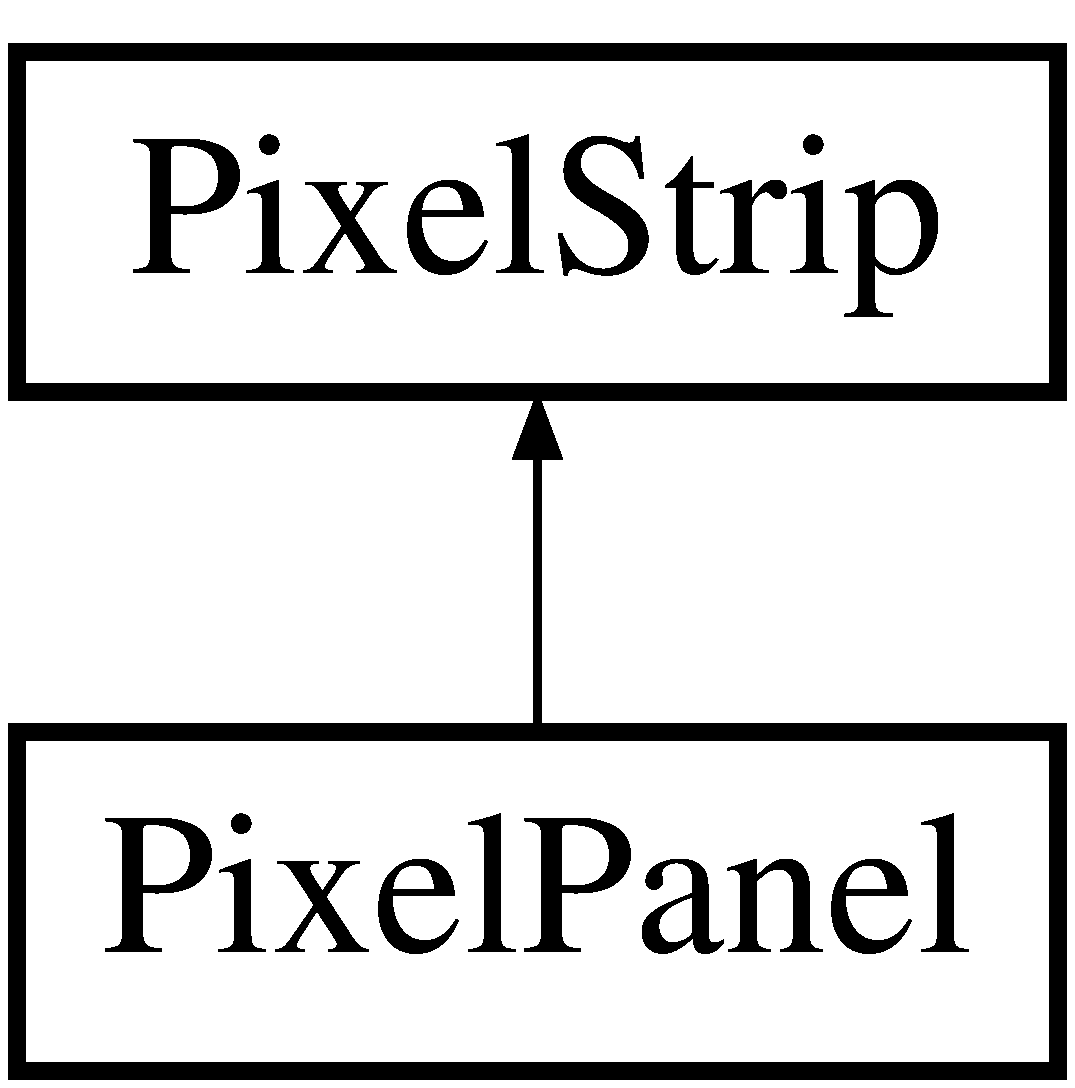
\includegraphics[height=2.000000cm]{class_pixel_panel}
\end{center}
\end{figure}
\subsection*{Public Member Functions}
\begin{DoxyCompactItemize}
\item 
{\bf Pixel\+Panel} ({\bf Pixel\+Strip} $\ast$strip, uint16\+\_\+t start\+Idx, uint16\+\_\+t {\bf num\+Pixels})
\item 
{\bf Pixel\+Strip} $\ast$ {\bf get\+Strip} ()
\item 
void {\bf set\+Pixel\+Color} (uint16\+\_\+t n, uint8\+\_\+t r, uint8\+\_\+t g, uint8\+\_\+t b)
\item 
void {\bf set\+Pixel\+Color} (uint16\+\_\+t n, uint32\+\_\+t c)
\item 
void {\bf clear} ()
\item 
uint16\+\_\+t {\bf num\+Pixels} (void) const 
\item 
uint32\+\_\+t {\bf get\+Pixel\+Color} (uint16\+\_\+t n) const 
\item 
uint16\+\_\+t {\bf get\+Offset} ()
\item 
void {\bf set\+Brightness} (uint8\+\_\+t b)
\item 
uint8\+\_\+t {\bf get\+Brightness} (void) const 
\end{DoxyCompactItemize}
\subsection*{Protected Attributes}
\begin{DoxyCompactItemize}
\item 
{\bf Pixel\+Strip} $\ast$ {\bf m\+\_\+strip}
\item 
uint16\+\_\+t {\bf m\+\_\+offset}
\item 
uint16\+\_\+t {\bf m\+\_\+num\+Pixels}
\item 
uint8\+\_\+t {\bf m\+\_\+brightness}
\end{DoxyCompactItemize}


\subsection{Detailed Description}
A pixel panel is a logical division of a physical \doxyref{Pixel\+Strip}{p.}{class_pixel_strip}. These are virtual panels, so multiple panels ccan be on a physical strip. 

\subsection{Constructor \& Destructor Documentation}
\index{Pixel\+Panel@{Pixel\+Panel}!Pixel\+Panel@{Pixel\+Panel}}
\index{Pixel\+Panel@{Pixel\+Panel}!Pixel\+Panel@{Pixel\+Panel}}
\subsubsection[{Pixel\+Panel}]{\setlength{\rightskip}{0pt plus 5cm}Pixel\+Panel\+::\+Pixel\+Panel (
\begin{DoxyParamCaption}
\item[{{\bf Pixel\+Strip} $\ast$}]{strip, }
\item[{uint16\+\_\+t}]{start\+Idx, }
\item[{uint16\+\_\+t}]{num\+Pixels}
\end{DoxyParamCaption}
)\hspace{0.3cm}{\ttfamily [inline]}}\label{class_pixel_panel_aa37805f359a7e5aa1db4654efcd3029c}
Create a logical panel inside a physical strip. 
\begin{DoxyParams}{Parameters}
{\em strip} & The physical pixel strip \\
\hline
{\em start\+Idx} & The starting pixl number on the physical device. Start at 0 for first pixel. \\
\hline
{\em num\+Pixels} & The number of pixels to reserve for this logical panel \\
\hline
\end{DoxyParams}


\subsection{Member Function Documentation}
\index{Pixel\+Panel@{Pixel\+Panel}!clear@{clear}}
\index{clear@{clear}!Pixel\+Panel@{Pixel\+Panel}}
\subsubsection[{clear}]{\setlength{\rightskip}{0pt plus 5cm}void Pixel\+Panel\+::clear (
\begin{DoxyParamCaption}
{}
\end{DoxyParamCaption}
)\hspace{0.3cm}{\ttfamily [inline]}, {\ttfamily [virtual]}}\label{class_pixel_panel_a0989d75f163e68d362e47d11695759e2}
Clear the panel (set to color 0 or dark) 

Implements {\bf Pixel\+Strip} \doxyref{}{p.}{class_pixel_strip_a9bc0c906bc3847c832e78af0c1afb6b8}.

\index{Pixel\+Panel@{Pixel\+Panel}!get\+Brightness@{get\+Brightness}}
\index{get\+Brightness@{get\+Brightness}!Pixel\+Panel@{Pixel\+Panel}}
\subsubsection[{get\+Brightness}]{\setlength{\rightskip}{0pt plus 5cm}uint8\+\_\+t Pixel\+Panel\+::get\+Brightness (
\begin{DoxyParamCaption}
\item[{void}]{}
\end{DoxyParamCaption}
) const\hspace{0.3cm}{\ttfamily [inline]}, {\ttfamily [virtual]}}\label{class_pixel_panel_ac9c071b78bb8b040a644e676ed1681fb}
Get the brightness of the strip \begin{DoxyReturn}{Returns}
0-\/255 where 0 is dark, 255 full brightness 
\end{DoxyReturn}


Implements {\bf Pixel\+Strip} \doxyref{}{p.}{class_pixel_strip_aa79c0e3c07e10f0c5c6cd4fb9d1a60ab}.

\index{Pixel\+Panel@{Pixel\+Panel}!get\+Offset@{get\+Offset}}
\index{get\+Offset@{get\+Offset}!Pixel\+Panel@{Pixel\+Panel}}
\subsubsection[{get\+Offset}]{\setlength{\rightskip}{0pt plus 5cm}uint16\+\_\+t Pixel\+Panel\+::get\+Offset (
\begin{DoxyParamCaption}
{}
\end{DoxyParamCaption}
)\hspace{0.3cm}{\ttfamily [inline]}}\label{class_pixel_panel_ae760cf40a15d724b58bd1e81f153361c}
Returns the offset of this logical panel in the physical strip. \begin{DoxyReturn}{Returns}
Pixel offset value 
\end{DoxyReturn}
\index{Pixel\+Panel@{Pixel\+Panel}!get\+Pixel\+Color@{get\+Pixel\+Color}}
\index{get\+Pixel\+Color@{get\+Pixel\+Color}!Pixel\+Panel@{Pixel\+Panel}}
\subsubsection[{get\+Pixel\+Color}]{\setlength{\rightskip}{0pt plus 5cm}uint32\+\_\+t Pixel\+Panel\+::get\+Pixel\+Color (
\begin{DoxyParamCaption}
\item[{uint16\+\_\+t}]{n}
\end{DoxyParamCaption}
) const\hspace{0.3cm}{\ttfamily [inline]}, {\ttfamily [virtual]}}\label{class_pixel_panel_a9b7aa3288daddef419e79530a4529dec}
Return the R\+G\+B color value in a particular pixel \begin{DoxyReturn}{Returns}
R\+G\+B color value 
\end{DoxyReturn}


Implements {\bf Pixel\+Strip} \doxyref{}{p.}{class_pixel_strip_a273498bf50216a646f24876da0e8d333}.

\index{Pixel\+Panel@{Pixel\+Panel}!get\+Strip@{get\+Strip}}
\index{get\+Strip@{get\+Strip}!Pixel\+Panel@{Pixel\+Panel}}
\subsubsection[{get\+Strip}]{\setlength{\rightskip}{0pt plus 5cm}{\bf Pixel\+Strip}$\ast$ Pixel\+Panel\+::get\+Strip (
\begin{DoxyParamCaption}
{}
\end{DoxyParamCaption}
)\hspace{0.3cm}{\ttfamily [inline]}}\label{class_pixel_panel_aa99dc12e0a4d684ceac285f9021cb88d}
Get the physical strip this panel is associated with \begin{DoxyReturn}{Returns}
Pointer to \doxyref{Pixel\+Strip}{p.}{class_pixel_strip} 
\end{DoxyReturn}
\index{Pixel\+Panel@{Pixel\+Panel}!num\+Pixels@{num\+Pixels}}
\index{num\+Pixels@{num\+Pixels}!Pixel\+Panel@{Pixel\+Panel}}
\subsubsection[{num\+Pixels}]{\setlength{\rightskip}{0pt plus 5cm}uint16\+\_\+t Pixel\+Panel\+::num\+Pixels (
\begin{DoxyParamCaption}
\item[{void}]{}
\end{DoxyParamCaption}
) const\hspace{0.3cm}{\ttfamily [inline]}, {\ttfamily [virtual]}}\label{class_pixel_panel_ade2c5c5942c0597ceff967cd5f44dbea}
Get the number of pixels in the panel \begin{DoxyReturn}{Returns}
Count of pixels 
\end{DoxyReturn}


Implements {\bf Pixel\+Strip} \doxyref{}{p.}{class_pixel_strip_a095201c971095020d1adc10b094c896f}.

\index{Pixel\+Panel@{Pixel\+Panel}!set\+Brightness@{set\+Brightness}}
\index{set\+Brightness@{set\+Brightness}!Pixel\+Panel@{Pixel\+Panel}}
\subsubsection[{set\+Brightness}]{\setlength{\rightskip}{0pt plus 5cm}void Pixel\+Panel\+::set\+Brightness (
\begin{DoxyParamCaption}
\item[{uint8\+\_\+t}]{b}
\end{DoxyParamCaption}
)\hspace{0.3cm}{\ttfamily [inline]}, {\ttfamily [virtual]}}\label{class_pixel_panel_a5c9e16717161c7230362f28aeccc82bb}
Set the brightness of the strip. 0 is lowest, 255 highest brightness 
\begin{DoxyParams}{Parameters}
{\em b} & Brightness value, 8 bit unsigned \\
\hline
\end{DoxyParams}


Implements {\bf Pixel\+Strip} \doxyref{}{p.}{class_pixel_strip_a3154e9d623c7ffc39dd70f6cfd39bd68}.

\index{Pixel\+Panel@{Pixel\+Panel}!set\+Pixel\+Color@{set\+Pixel\+Color}}
\index{set\+Pixel\+Color@{set\+Pixel\+Color}!Pixel\+Panel@{Pixel\+Panel}}
\subsubsection[{set\+Pixel\+Color}]{\setlength{\rightskip}{0pt plus 5cm}void Pixel\+Panel\+::set\+Pixel\+Color (
\begin{DoxyParamCaption}
\item[{uint16\+\_\+t}]{n, }
\item[{uint8\+\_\+t}]{r, }
\item[{uint8\+\_\+t}]{g, }
\item[{uint8\+\_\+t}]{b}
\end{DoxyParamCaption}
)\hspace{0.3cm}{\ttfamily [inline]}, {\ttfamily [virtual]}}\label{class_pixel_panel_aab3e27324193de4990b9db69c2f31dfe}
Set a specific pixel to the r,g,b color value. 
\begin{DoxyParams}{Parameters}
{\em n} & Pixel number \\
\hline
{\em r} & Red component \\
\hline
{\em g} & Green component \\
\hline
{\em b} & Blue component \\
\hline
\end{DoxyParams}


Implements {\bf Pixel\+Strip} \doxyref{}{p.}{class_pixel_strip_a391a297d5f9faf1be384bada7199acce}.

\index{Pixel\+Panel@{Pixel\+Panel}!set\+Pixel\+Color@{set\+Pixel\+Color}}
\index{set\+Pixel\+Color@{set\+Pixel\+Color}!Pixel\+Panel@{Pixel\+Panel}}
\subsubsection[{set\+Pixel\+Color}]{\setlength{\rightskip}{0pt plus 5cm}void Pixel\+Panel\+::set\+Pixel\+Color (
\begin{DoxyParamCaption}
\item[{uint16\+\_\+t}]{n, }
\item[{uint32\+\_\+t}]{c}
\end{DoxyParamCaption}
)\hspace{0.3cm}{\ttfamily [inline]}, {\ttfamily [virtual]}}\label{class_pixel_panel_a1e25c5aed5eea466b1e4e3c6adcbc8c1}
Set a specific pixel to the R\+G\+B color value. 
\begin{DoxyParams}{Parameters}
{\em n} & Pixel number \\
\hline
{\em c} & R\+G\+B Color \\
\hline
\end{DoxyParams}


Implements {\bf Pixel\+Strip} \doxyref{}{p.}{class_pixel_strip_a8fac5124e323b48aaa854143d0d91922}.



\subsection{Member Data Documentation}
\index{Pixel\+Panel@{Pixel\+Panel}!m\+\_\+brightness@{m\+\_\+brightness}}
\index{m\+\_\+brightness@{m\+\_\+brightness}!Pixel\+Panel@{Pixel\+Panel}}
\subsubsection[{m\+\_\+brightness}]{\setlength{\rightskip}{0pt plus 5cm}uint8\+\_\+t Pixel\+Panel\+::m\+\_\+brightness\hspace{0.3cm}{\ttfamily [protected]}}\label{class_pixel_panel_ae1d6c1677dc1ffda25a04e1d00dac4f4}
current brightness level for this logical panel \index{Pixel\+Panel@{Pixel\+Panel}!m\+\_\+num\+Pixels@{m\+\_\+num\+Pixels}}
\index{m\+\_\+num\+Pixels@{m\+\_\+num\+Pixels}!Pixel\+Panel@{Pixel\+Panel}}
\subsubsection[{m\+\_\+num\+Pixels}]{\setlength{\rightskip}{0pt plus 5cm}uint16\+\_\+t Pixel\+Panel\+::m\+\_\+num\+Pixels\hspace{0.3cm}{\ttfamily [protected]}}\label{class_pixel_panel_ab6d0c54bcdab907d3bb955179e40a798}
total pixels in this logical panel \index{Pixel\+Panel@{Pixel\+Panel}!m\+\_\+offset@{m\+\_\+offset}}
\index{m\+\_\+offset@{m\+\_\+offset}!Pixel\+Panel@{Pixel\+Panel}}
\subsubsection[{m\+\_\+offset}]{\setlength{\rightskip}{0pt plus 5cm}uint16\+\_\+t Pixel\+Panel\+::m\+\_\+offset\hspace{0.3cm}{\ttfamily [protected]}}\label{class_pixel_panel_a92c44f1faf2558f55221294694d06799}
starting pixel number in strip \index{Pixel\+Panel@{Pixel\+Panel}!m\+\_\+strip@{m\+\_\+strip}}
\index{m\+\_\+strip@{m\+\_\+strip}!Pixel\+Panel@{Pixel\+Panel}}
\subsubsection[{m\+\_\+strip}]{\setlength{\rightskip}{0pt plus 5cm}{\bf Pixel\+Strip}$\ast$ Pixel\+Panel\+::m\+\_\+strip\hspace{0.3cm}{\ttfamily [protected]}}\label{class_pixel_panel_adc25dceb1b6c46d575873bcb66cb6fb9}
Pointer to the physical strip 

The documentation for this class was generated from the following file\+:\begin{DoxyCompactItemize}
\item 
C\+:/\+Users/\+Russell/\+Documents/\+Arduino/libraries/\+Opcom\+\_\+\+Neo\+Pixel/Pixel\+Panel.\+h\end{DoxyCompactItemize}

\section{Pixel\+Strip Class Reference}
\label{class_pixel_strip}\index{Pixel\+Strip@{Pixel\+Strip}}


{\ttfamily \#include $<$Pixel\+Strip.\+h$>$}

Inheritance diagram for Pixel\+Strip\+:\begin{figure}[H]
\begin{center}
\leavevmode
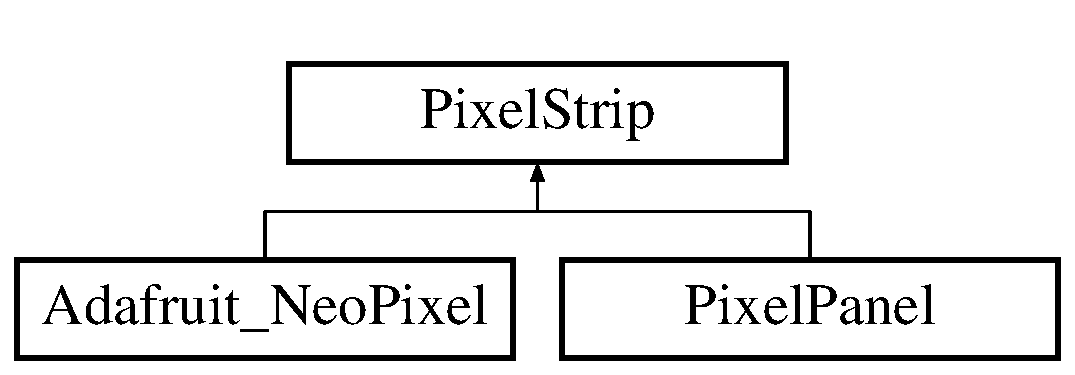
\includegraphics[height=2.000000cm]{class_pixel_strip}
\end{center}
\end{figure}
\subsection*{Public Member Functions}
\begin{DoxyCompactItemize}
\item 
virtual void {\bf set\+Pixel\+Color} (uint16\+\_\+t n, uint8\+\_\+t r, uint8\+\_\+t g, uint8\+\_\+t b)=0
\item 
virtual void {\bf set\+Pixel\+Color} (uint16\+\_\+t n, uint32\+\_\+t c)=0
\item 
virtual void {\bf clear} ()=0
\item 
virtual uint16\+\_\+t {\bf num\+Pixels} (void) const =0
\item 
virtual uint32\+\_\+t {\bf get\+Pixel\+Color} (uint16\+\_\+t n) const =0
\item 
virtual uint8\+\_\+t {\bf get\+Brightness} (void) const =0
\item 
virtual void {\bf set\+Brightness} (uint8\+\_\+t b)=0
\item 
virtual void {\bf set\+All\+Pixels} (uint32\+\_\+t color)
\end{DoxyCompactItemize}


\subsection{Detailed Description}
A virtual base class for any sort of strip of led pixels. This is a physical implementation, so this class represents the actual physical device. 

\subsection{Member Function Documentation}
\index{Pixel\+Strip@{Pixel\+Strip}!clear@{clear}}
\index{clear@{clear}!Pixel\+Strip@{Pixel\+Strip}}
\subsubsection[{clear}]{\setlength{\rightskip}{0pt plus 5cm}virtual void Pixel\+Strip\+::clear (
\begin{DoxyParamCaption}
{}
\end{DoxyParamCaption}
)\hspace{0.3cm}{\ttfamily [pure virtual]}}\label{class_pixel_strip_a9bc0c906bc3847c832e78af0c1afb6b8}
Clear the panel (set to color 0 or dark) 

Implemented in {\bf Adafruit\+\_\+\+Neo\+Pixel} \doxyref{}{p.}{class_adafruit___neo_pixel_ac06a711d7bf63bada61b52a1d528e4b4}, and {\bf Pixel\+Panel} \doxyref{}{p.}{class_pixel_panel_a0989d75f163e68d362e47d11695759e2}.

\index{Pixel\+Strip@{Pixel\+Strip}!get\+Brightness@{get\+Brightness}}
\index{get\+Brightness@{get\+Brightness}!Pixel\+Strip@{Pixel\+Strip}}
\subsubsection[{get\+Brightness}]{\setlength{\rightskip}{0pt plus 5cm}virtual uint8\+\_\+t Pixel\+Strip\+::get\+Brightness (
\begin{DoxyParamCaption}
\item[{void}]{}
\end{DoxyParamCaption}
) const\hspace{0.3cm}{\ttfamily [pure virtual]}}\label{class_pixel_strip_aa79c0e3c07e10f0c5c6cd4fb9d1a60ab}
Get the brightness of the strip \begin{DoxyReturn}{Returns}
0-\/255 where 0 is dark, 255 full brightness 
\end{DoxyReturn}


Implemented in {\bf Pixel\+Panel} \doxyref{}{p.}{class_pixel_panel_ac9c071b78bb8b040a644e676ed1681fb}, and {\bf Adafruit\+\_\+\+Neo\+Pixel} \doxyref{}{p.}{class_adafruit___neo_pixel_a3e3dc79b4fad55ea34799c6fa5f8cb82}.

\index{Pixel\+Strip@{Pixel\+Strip}!get\+Pixel\+Color@{get\+Pixel\+Color}}
\index{get\+Pixel\+Color@{get\+Pixel\+Color}!Pixel\+Strip@{Pixel\+Strip}}
\subsubsection[{get\+Pixel\+Color}]{\setlength{\rightskip}{0pt plus 5cm}virtual uint32\+\_\+t Pixel\+Strip\+::get\+Pixel\+Color (
\begin{DoxyParamCaption}
\item[{uint16\+\_\+t}]{n}
\end{DoxyParamCaption}
) const\hspace{0.3cm}{\ttfamily [pure virtual]}}\label{class_pixel_strip_a273498bf50216a646f24876da0e8d333}
Return the R\+G\+B color value in a particular pixel \begin{DoxyReturn}{Returns}
R\+G\+B color value 
\end{DoxyReturn}


Implemented in {\bf Adafruit\+\_\+\+Neo\+Pixel} \doxyref{}{p.}{class_adafruit___neo_pixel_a309cd3fb7a3e2e87a26e7a2fcf6391f1}, and {\bf Pixel\+Panel} \doxyref{}{p.}{class_pixel_panel_a9b7aa3288daddef419e79530a4529dec}.

\index{Pixel\+Strip@{Pixel\+Strip}!num\+Pixels@{num\+Pixels}}
\index{num\+Pixels@{num\+Pixels}!Pixel\+Strip@{Pixel\+Strip}}
\subsubsection[{num\+Pixels}]{\setlength{\rightskip}{0pt plus 5cm}virtual uint16\+\_\+t Pixel\+Strip\+::num\+Pixels (
\begin{DoxyParamCaption}
\item[{void}]{}
\end{DoxyParamCaption}
) const\hspace{0.3cm}{\ttfamily [pure virtual]}}\label{class_pixel_strip_a095201c971095020d1adc10b094c896f}
Get the number of pixels in the panel \begin{DoxyReturn}{Returns}
Count of pixels 
\end{DoxyReturn}


Implemented in {\bf Adafruit\+\_\+\+Neo\+Pixel} \doxyref{}{p.}{class_adafruit___neo_pixel_a2b2ec05493af8de2a6afe63c1e8f9516}, and {\bf Pixel\+Panel} \doxyref{}{p.}{class_pixel_panel_ade2c5c5942c0597ceff967cd5f44dbea}.

\index{Pixel\+Strip@{Pixel\+Strip}!set\+All\+Pixels@{set\+All\+Pixels}}
\index{set\+All\+Pixels@{set\+All\+Pixels}!Pixel\+Strip@{Pixel\+Strip}}
\subsubsection[{set\+All\+Pixels}]{\setlength{\rightskip}{0pt plus 5cm}virtual void Pixel\+Strip\+::set\+All\+Pixels (
\begin{DoxyParamCaption}
\item[{uint32\+\_\+t}]{color}
\end{DoxyParamCaption}
)\hspace{0.3cm}{\ttfamily [inline]}, {\ttfamily [virtual]}}\label{class_pixel_strip_ac5811b15226d348a3c64d7a5498128e2}
Set all the leds to a single color. show() must be called to take effect. 
\begin{DoxyParams}{Parameters}
{\em color} & The color to set all leds to \\
\hline
\end{DoxyParams}
\index{Pixel\+Strip@{Pixel\+Strip}!set\+Brightness@{set\+Brightness}}
\index{set\+Brightness@{set\+Brightness}!Pixel\+Strip@{Pixel\+Strip}}
\subsubsection[{set\+Brightness}]{\setlength{\rightskip}{0pt plus 5cm}virtual void Pixel\+Strip\+::set\+Brightness (
\begin{DoxyParamCaption}
\item[{uint8\+\_\+t}]{b}
\end{DoxyParamCaption}
)\hspace{0.3cm}{\ttfamily [pure virtual]}}\label{class_pixel_strip_a3154e9d623c7ffc39dd70f6cfd39bd68}
Set the brightness of the strip. 0 is lowest, 255 highest brightness 
\begin{DoxyParams}{Parameters}
{\em b} & Brightness value, 8 bit unsigned \\
\hline
\end{DoxyParams}


Implemented in {\bf Adafruit\+\_\+\+Neo\+Pixel} \doxyref{}{p.}{class_adafruit___neo_pixel_a06915c54a2cc307763b3c44a601229ba}, and {\bf Pixel\+Panel} \doxyref{}{p.}{class_pixel_panel_a5c9e16717161c7230362f28aeccc82bb}.

\index{Pixel\+Strip@{Pixel\+Strip}!set\+Pixel\+Color@{set\+Pixel\+Color}}
\index{set\+Pixel\+Color@{set\+Pixel\+Color}!Pixel\+Strip@{Pixel\+Strip}}
\subsubsection[{set\+Pixel\+Color}]{\setlength{\rightskip}{0pt plus 5cm}virtual void Pixel\+Strip\+::set\+Pixel\+Color (
\begin{DoxyParamCaption}
\item[{uint16\+\_\+t}]{n, }
\item[{uint8\+\_\+t}]{r, }
\item[{uint8\+\_\+t}]{g, }
\item[{uint8\+\_\+t}]{b}
\end{DoxyParamCaption}
)\hspace{0.3cm}{\ttfamily [pure virtual]}}\label{class_pixel_strip_a391a297d5f9faf1be384bada7199acce}
Set a specific pixel to the r,g,b color value. 
\begin{DoxyParams}{Parameters}
{\em n} & Pixel number \\
\hline
{\em r} & Red component \\
\hline
{\em g} & Green component \\
\hline
{\em b} & Blue component \\
\hline
\end{DoxyParams}


Implemented in {\bf Adafruit\+\_\+\+Neo\+Pixel} \doxyref{}{p.}{class_adafruit___neo_pixel_ab8763ccc6f9a090df1f753905fd5561e}, and {\bf Pixel\+Panel} \doxyref{}{p.}{class_pixel_panel_aab3e27324193de4990b9db69c2f31dfe}.

\index{Pixel\+Strip@{Pixel\+Strip}!set\+Pixel\+Color@{set\+Pixel\+Color}}
\index{set\+Pixel\+Color@{set\+Pixel\+Color}!Pixel\+Strip@{Pixel\+Strip}}
\subsubsection[{set\+Pixel\+Color}]{\setlength{\rightskip}{0pt plus 5cm}virtual void Pixel\+Strip\+::set\+Pixel\+Color (
\begin{DoxyParamCaption}
\item[{uint16\+\_\+t}]{n, }
\item[{uint32\+\_\+t}]{c}
\end{DoxyParamCaption}
)\hspace{0.3cm}{\ttfamily [pure virtual]}}\label{class_pixel_strip_a8fac5124e323b48aaa854143d0d91922}
Set a specific pixel to the R\+G\+B color value. 
\begin{DoxyParams}{Parameters}
{\em n} & Pixel number \\
\hline
{\em c} & R\+G\+B Color \\
\hline
\end{DoxyParams}


Implemented in {\bf Adafruit\+\_\+\+Neo\+Pixel} \doxyref{}{p.}{class_adafruit___neo_pixel_a19fc274330c0e65907929ee03b93b1c3}, and {\bf Pixel\+Panel} \doxyref{}{p.}{class_pixel_panel_a1e25c5aed5eea466b1e4e3c6adcbc8c1}.



The documentation for this class was generated from the following file\+:\begin{DoxyCompactItemize}
\item 
C\+:/\+Users/\+Russell/\+Documents/\+Arduino/libraries/\+Opcom\+\_\+\+Neo\+Pixel/Pixel\+Strip.\+h\end{DoxyCompactItemize}

\section{Opcom\+:\+:Timer Class Reference}
\label{class_opcom_1_1_timer}\index{Opcom\+::\+Timer@{Opcom\+::\+Timer}}


{\ttfamily \#include $<$Timer.\+h$>$}

\subsection*{Public Member Functions}
\begin{DoxyCompactItemize}
\item 
{\bf Timer} (unsigned long ms)
\item 
bool {\bf is\+Expired} ()
\item 
void {\bf reset} ()
\item 
void {\bf set\+Interval} (unsigned long ms)
\item 
bool {\bf has\+Period\+Passed} ()
\end{DoxyCompactItemize}


\subsection{Detailed Description}
A timer class. 

\subsection{Constructor \& Destructor Documentation}
\index{Opcom\+::\+Timer@{Opcom\+::\+Timer}!Timer@{Timer}}
\index{Timer@{Timer}!Opcom\+::\+Timer@{Opcom\+::\+Timer}}
\subsubsection[{Timer}]{\setlength{\rightskip}{0pt plus 5cm}Opcom\+::\+Timer\+::\+Timer (
\begin{DoxyParamCaption}
\item[{unsigned long}]{ms}
\end{DoxyParamCaption}
)\hspace{0.3cm}{\ttfamily [inline]}}\label{class_opcom_1_1_timer_ab827892cc7e976d115926edd95fdd6bf}
Create a timer with a specific interval 
\begin{DoxyParams}{Parameters}
{\em ms} & Time in milliseconds \\
\hline
\end{DoxyParams}


\subsection{Member Function Documentation}
\index{Opcom\+::\+Timer@{Opcom\+::\+Timer}!has\+Period\+Passed@{has\+Period\+Passed}}
\index{has\+Period\+Passed@{has\+Period\+Passed}!Opcom\+::\+Timer@{Opcom\+::\+Timer}}
\subsubsection[{has\+Period\+Passed}]{\setlength{\rightskip}{0pt plus 5cm}bool Opcom\+::\+Timer\+::has\+Period\+Passed (
\begin{DoxyParamCaption}
{}
\end{DoxyParamCaption}
)\hspace{0.3cm}{\ttfamily [inline]}}\label{class_opcom_1_1_timer_a1f20e8351d1a9fb0d97326b54d8ee380}
Check if expired, and reset if so. Using this method, the timer will prevent drifting by adding any extra time it took between calls. After a call to this method, when it returns true, it also does a reset of the timer. \begin{DoxyReturn}{Returns}
True if the timer period has elapsed. 
\end{DoxyReturn}
\index{Opcom\+::\+Timer@{Opcom\+::\+Timer}!is\+Expired@{is\+Expired}}
\index{is\+Expired@{is\+Expired}!Opcom\+::\+Timer@{Opcom\+::\+Timer}}
\subsubsection[{is\+Expired}]{\setlength{\rightskip}{0pt plus 5cm}bool Opcom\+::\+Timer\+::is\+Expired (
\begin{DoxyParamCaption}
{}
\end{DoxyParamCaption}
)\hspace{0.3cm}{\ttfamily [inline]}}\label{class_opcom_1_1_timer_a03397c57a09388588d139300e5e78975}
Check if the interval has passed. \begin{DoxyReturn}{Returns}
true if the interval has passed 
\end{DoxyReturn}
\index{Opcom\+::\+Timer@{Opcom\+::\+Timer}!reset@{reset}}
\index{reset@{reset}!Opcom\+::\+Timer@{Opcom\+::\+Timer}}
\subsubsection[{reset}]{\setlength{\rightskip}{0pt plus 5cm}void Opcom\+::\+Timer\+::reset (
\begin{DoxyParamCaption}
{}
\end{DoxyParamCaption}
)\hspace{0.3cm}{\ttfamily [inline]}}\label{class_opcom_1_1_timer_af27be36621d5a80d5a20c1f32a3ab632}
Reset the start time to the current time \index{Opcom\+::\+Timer@{Opcom\+::\+Timer}!set\+Interval@{set\+Interval}}
\index{set\+Interval@{set\+Interval}!Opcom\+::\+Timer@{Opcom\+::\+Timer}}
\subsubsection[{set\+Interval}]{\setlength{\rightskip}{0pt plus 5cm}void Opcom\+::\+Timer\+::set\+Interval (
\begin{DoxyParamCaption}
\item[{unsigned long}]{ms}
\end{DoxyParamCaption}
)\hspace{0.3cm}{\ttfamily [inline]}}\label{class_opcom_1_1_timer_ac3481c346fdf0a1c3dd64ecda9c06370}
Change the interval of the timer 
\begin{DoxyParams}{Parameters}
{\em ms} & \doxyref{Timer}{p.}{class_opcom_1_1_timer} interval in milliseconds \\
\hline
\end{DoxyParams}


The documentation for this class was generated from the following file\+:\begin{DoxyCompactItemize}
\item 
C\+:/\+Users/\+Russell/\+Documents/\+Arduino/libraries/\+Opcom\+\_\+\+Neo\+Pixel/Timer.\+h\end{DoxyCompactItemize}

%--- End generated contents ---

% Index
\backmatter
\newpage
\phantomsection
\clearemptydoublepage
\addcontentsline{toc}{chapter}{Index}
\printindex

\end{document}
